\begin{frame}{}
	\maketitle
\end{frame}
\note[itemize]{
	\item Una de las mejores historias del ciclo de Conan
	\item Una de las mejores historias de REH
	\item Uno de mis relatos favoritos, tal vez mi relato favorito del ciclo de Conan.
}

\begin{frame}{La torre del elefante}
\begin{columns}
\column[t]{0.5\textwidth}
 \begin{figure}[htb]
  \centering
  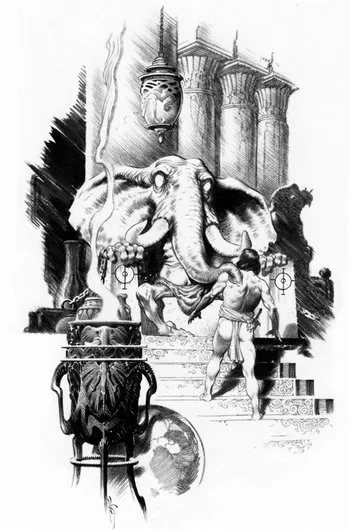
\includegraphics[width=0.4\textwidth]{img/Intro}
  \caption{Mark Schultz}
\end{figure}
\column[t]{0.5\textwidth}
     \begin{itemize}
         \item Una historia corta de Robert E. Howard
         \item Una de sus mejores historias
         \item Espada y hechicería (Espada y brujería) pura
     \end{itemize}
\end{columns}
\end{frame}
\note[itemize]{
	\item Voy a dar crédito a los artistas cuando no sea evidente
	\item Es la historia de espada y hechicería por antonomasia
	\item Explicar espada y hechicería vs espada y brujería
}

\begin{frame}{Publicación}
\begin{columns}
\column[t]{0.4\textwidth}
    \begin{figure}[htb]
    \centering
        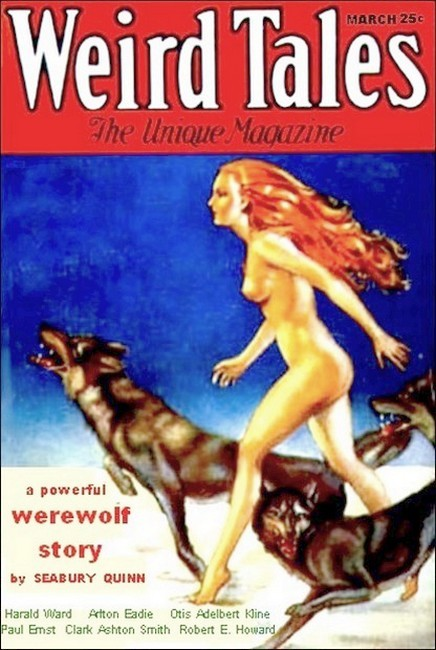
\includegraphics[width=0.5\textwidth]{img/WeirdTales-1933-03}
        \caption{Marzo de 1933}
    \end{figure}
\column[t]{0.6\textwidth}
    \begin{itemize}
         \item Publicada por primera vez en Weird Tales
         \item Alrededor de unas 20 páginas
         \begin{itemize}
            \item 9800 palabras en Ingles
            \item 10600 palabras en Español
            \item Lectura en 60-90 minutos
         \end{itemize}
         \item Una historia de su personaje mas famoso: Conan el bárbaro
         \item Muchas veces publicada en Español y en el idioma original
    \end{itemize}
\end{columns}
\end{frame}
\note[itemize]{
	\item La historia se encuentra en muchas recopilaciones y en varias ediciones tanto en Inglés como en Español
	\item Ésta es la historia que yo siempre recomiendo a alguien que nunca ha leido al Conan de REH
}

\begin{frame}{La primera ilustración}
	\begin{columns}
		\column[t]{0.4\textwidth}
		\begin{figure}[htb]
			\centering
			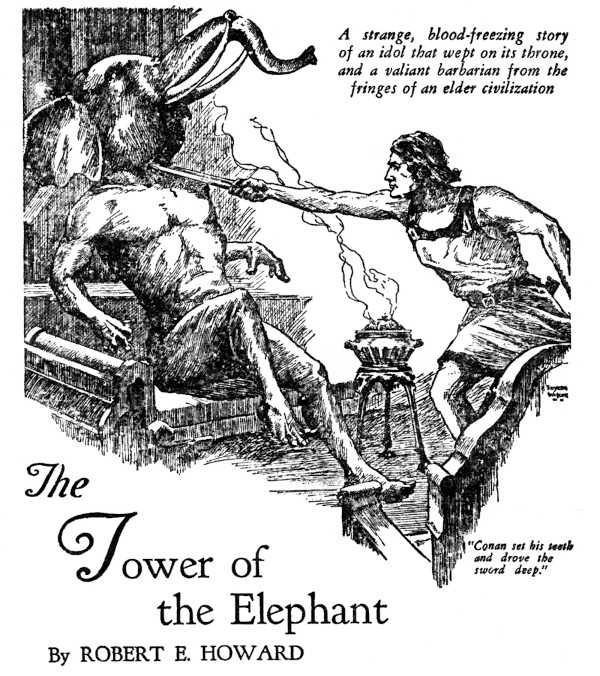
\includegraphics[width=0.75\textwidth]{img/JayemWilcoxTowerOfTheElephant}
			\caption{Jayem Wilcox}
		\end{figure}
		\column[t]{0.6\textwidth}
		\begin{itemize}
			\item Esta ilustración acompaña a la primera edición de la historia
		\end{itemize}
	\end{columns}
\end{frame}
\note[itemize]{
	\item Muchos ilustradores dibujan alguna escena de esta historia para sus portafolios
	\item Ésta fue la primera ilustración del relato
	\item Esto se vuelve interesante por una controversia aue explicare mas adelante
}

\begin{frame}{Orden de publicación del ciclo de Conan}
\begin{figure}[htb]
  \centering
  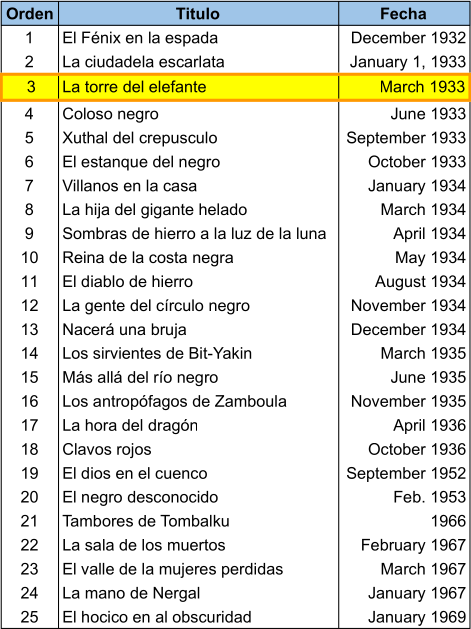
\includegraphics[width=0.32\textwidth]{img/OrdenPublicacion}
\end{figure}
\end{frame}
\note[itemize]{
	\item La torre del elefante forma parte del ciclo de Conan, que consta de 18 a 25 historias de REH, dependiendo de cómo queramos contarlas.
	\item Si solo se cuentan historias publicadas en la vida de REH, son 18 (o 17 dependiendo de si se cuenta o no \say{La hija del gigante helado}).
	\item Si se añaden la historias que fueron rechazadas por los editores durante la vida de REH, y luego publicadas después de su muerte; así como fragmentos que el autor dejó inconclusos y que fueron --muchos años después-- terminados y publicados por otros autores, ahí la cuenta sube a 25.
}

\begin{frame}{Cronología ficticia del personaje}
\begin{figure}[htb]
  \centering
  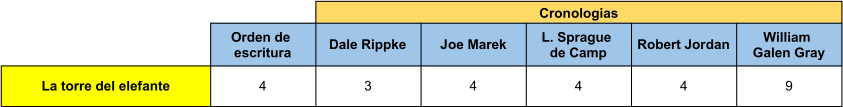
\includegraphics[width=0.85\textwidth]{img/Cronollogias}
\end{figure}
\end{frame}
\note[itemize]{
	\item Ha habido varios intentos de establecer una cronología de la vida ficticia de Conan. De estos intentos el más famoso es el de Miller/Clark/de Camp, porque contó con la bendición de REH en su versión más temprana.
	\item Aunque hay por los menos otros cuatro intentos importantes, que ya incluyen los trabajos de los otros autores escritos muchos años después de la muerte de REH.
	\item Casi todas las cronologías coinciden en que este debería ser el segundo *relato* de Conan, (de los escritos por REH), en el orden de la vida del personaje.
	\item Es decir, donde nos encontramos con un Conan muy joven. Aunque en el relato su edad no se menciona, de acuerdo a las cronologías Conan deberia haber tenido cerca de 17 años.
	\item De las otras obras originales de REH anteriores en la cronología dos no son cuentos.
	\item El ensayo La era Hiboria y el poema Cimeria.
	\item Finalmente a la única historia que la antecede: La hija del gigante helado a veces se le disputa su status de historia de Conan.
}

\begin{frame}{Espacio en la edad Hiboria}
\begin{figure}[htp]
 \centering
 \begin{subfigure}[b]{0.48\textwidth}
   \includegraphics[width=\textwidth]{img/mapas/todo}
   %\caption{Barry Windsor Smith}
 \end{subfigure}
~
 \begin{subfigure}[b]{0.48\textwidth}
   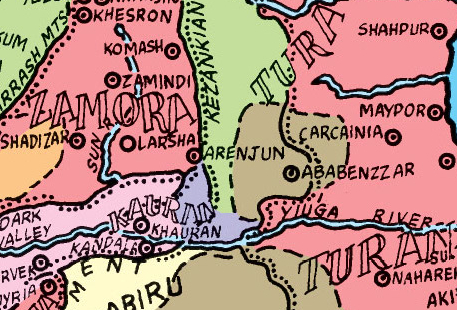
\includegraphics[width=\textwidth]{img/mapas/inset}
   %\caption{Silvio \say{Sal} Buscema}
 \end{subfigure}
 \caption{La ciudad de Arenjun en la provincia de Zamora. La \say{ciudad de los ladrones}}
 \end{figure}
\end{frame}
\note[itemize]{
	\item De nuevo en la historia jamás se menciona el nombre de la ciudad en donde sucede la aventura.
	\item Pero si se analiza la obra de REH en conjunto y en particular con la cronología avanzada de Conan. La mayoría está de acuerdo de que tuvo que pasar en Arejun una ciudad de la provincia de Zamora
	\item REH, no dejo un mapa oficial de la era hiboria, pero deja constancia de que si había dibujado un mapa y que cuando vio el mapa que le mandaron Miller y Clark; REH mencionó que su mapa y el de ellos era muy parecido
	\item Entonces tomando en cuenta que todo esto es una geografía imaginaria, y que además fue en su mayoría creada años después de muerte de su autor original, por mucho estudiosos de la obra, es decir tomen todo esto con un granito de sal.
	\item Habiendo dicho esto si hay como que un consenso general en que el mapa debe ser algo como este.
}

\section{Adaptaciones}
\note[itemize]{
	\item Hablar de la importancia de los comics en Conan, y como han sido los únicos medios en los que se ha adaptado la obra original de Howard
	\item Películas y videojuegos han usado el mundo creado por Howard, la era hiboria pero han hecho historias aparte.
}

\begin{frame}{Conan the barbarian}
\begin{columns}
\column[t]{0.4\textwidth}
    \begin{figure}[htb]
    \centering
        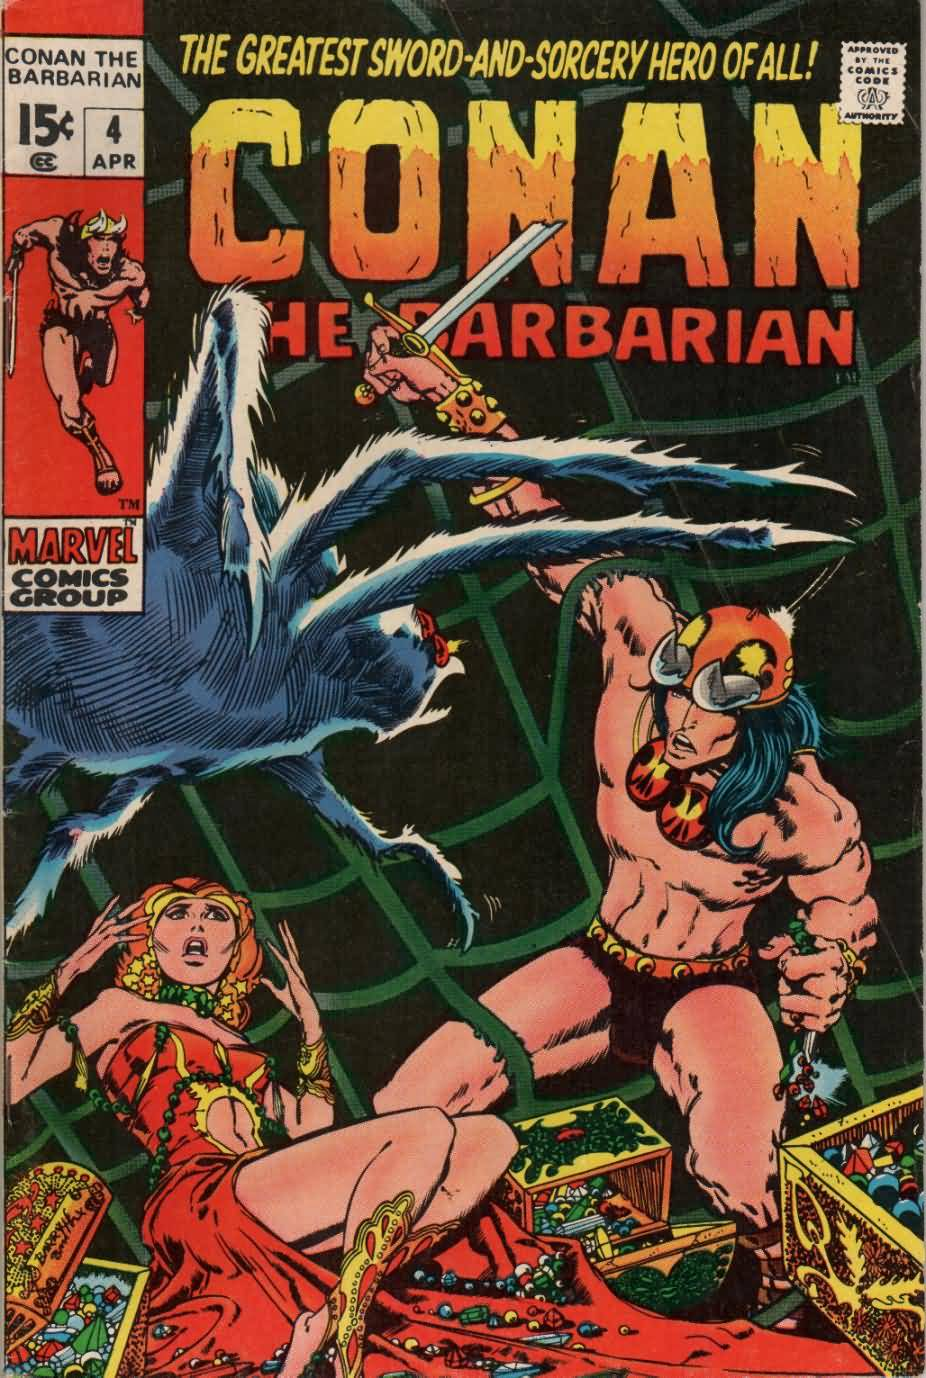
\includegraphics[width=0.55\textwidth]{img/TheBarbarian004Portada}
        \caption{26 de Enero de 1971}
    \end{figure}
\column[t]{0.6\textwidth}
    \begin{itemize}
         \item Número 4 en la serie
         \item 21 páginas
         \item Créditos:
         \begin{description}
            \item[Dibujante:] Barry Windsor Smith
            \item[Entintador:] Silvio \say{Sal} Buscema
            \item[Escritor:] Roy Thomas
            \item[Letrista:] Sam Rosen
            \item[Editor:] Stand Lee
         \end{description}
    \end{itemize}
\end{columns}
\end{frame}
\note[itemize]{
	\item En el canal de MKV, él dice que este es uno de los mejores cómics, no solo de Conan, ni de Marvel sino de su época de la década de los 70s.
	\item El dibujante e ilustrado Ingles Barry Windsor Smith, se volvio famoso por su trabajo en este titulo entre 1970 y 1973, despues dibujaria Weapon X.
	\item El dibujante Italoamericano Sal Buscema, entitno en uno de sus primeros trabajos (antes de que se volviera artista principal).
	\item Roy Thomas, es quein introdujo el personaje de Coonan a los comics, es probablemente el mejor adaptador de historias de REH al Comic. Ha creado muchisimos peronajes de Marvel, probablemente la figura mas influyente de Marvel despues de Stand Lee.
	\item Se le da credito como editor al jefe de la compania Satand Lee
}

% \begin{frame}{}
% \begin{figure}[htp]
%  \centering
%  \begin{subfigure}[b]{0.16\textwidth}
%    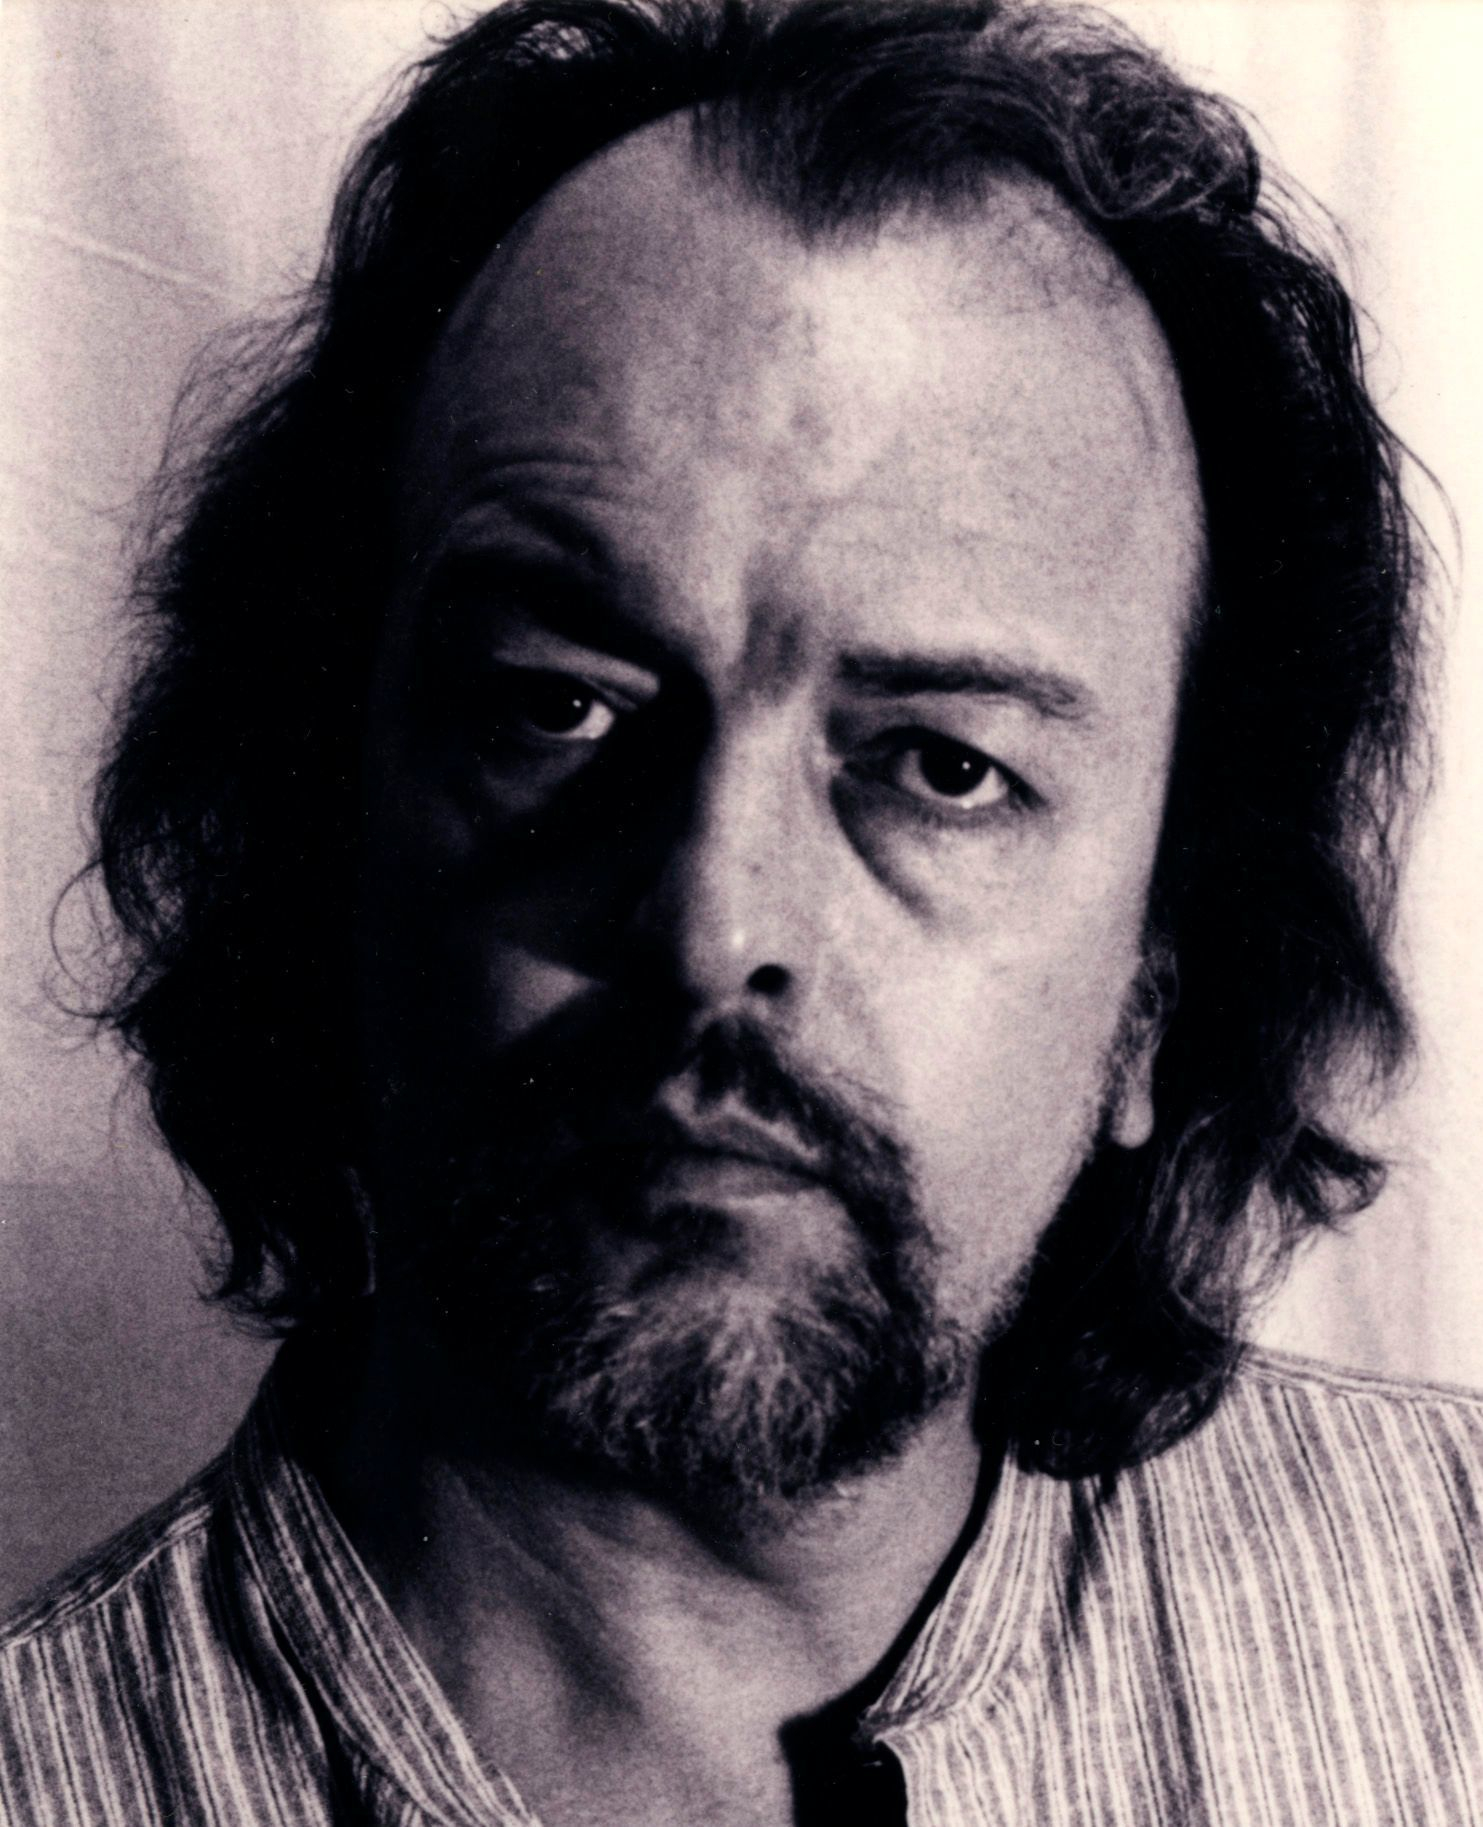
\includegraphics[width=\textwidth]{img/artistas/BarryWindsorSmith}
%    \caption{Barry Windsor Smith}
%  \end{subfigure}
% ~
%  \begin{subfigure}[b]{0.16\textwidth}
%    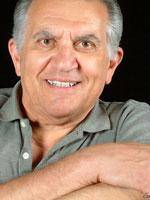
\includegraphics[width=\textwidth]{img/artistas/SalBuscema}
%    \caption{Silvio \say{Sal} Buscema}
%  \end{subfigure}
%  ~
%  \begin{subfigure}[b]{0.16\textwidth}
%    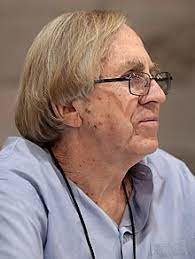
\includegraphics[width=\textwidth]{img/artistas/RoyThomas}
%    \caption{Roy Thomas}
%  \end{subfigure}
% ~
%  \begin{subfigure}[b]{0.16\textwidth}
%    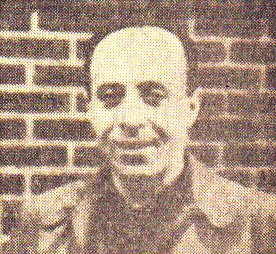
\includegraphics[width=\textwidth]{img/artistas/SamRosen1964}
%    \caption{Sam Rosen}
%  \end{subfigure}
% ~
%  \begin{subfigure}[b]{0.16\textwidth}
%    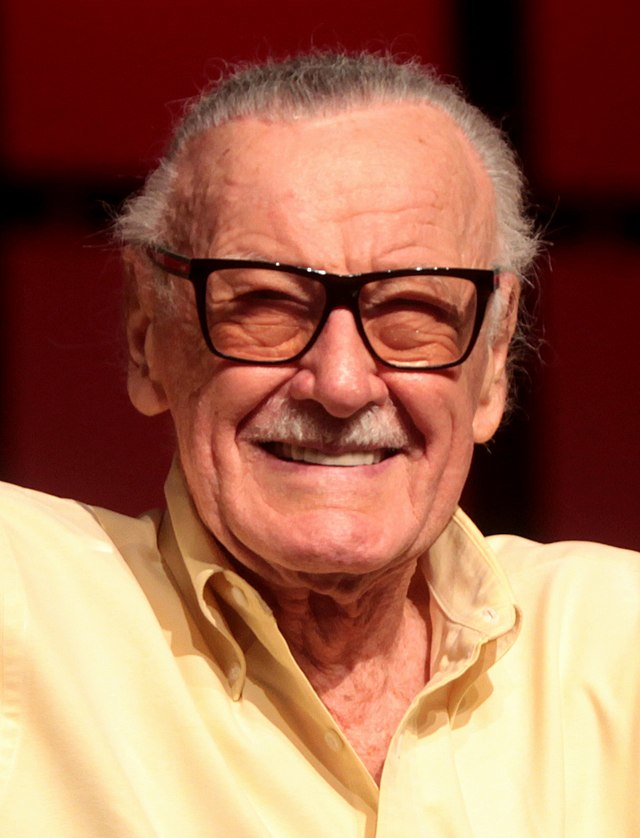
\includegraphics[width=\textwidth]{img/artistas/StanLee}
%    \caption{Stand Lee}
%  \end{subfigure}
% \end{figure}
% \end{frame}


\begin{frame}{The savage sword of Conan}
\begin{columns}
\column[t]{0.4\textwidth}
    \begin{figure}[htb]
    \centering
        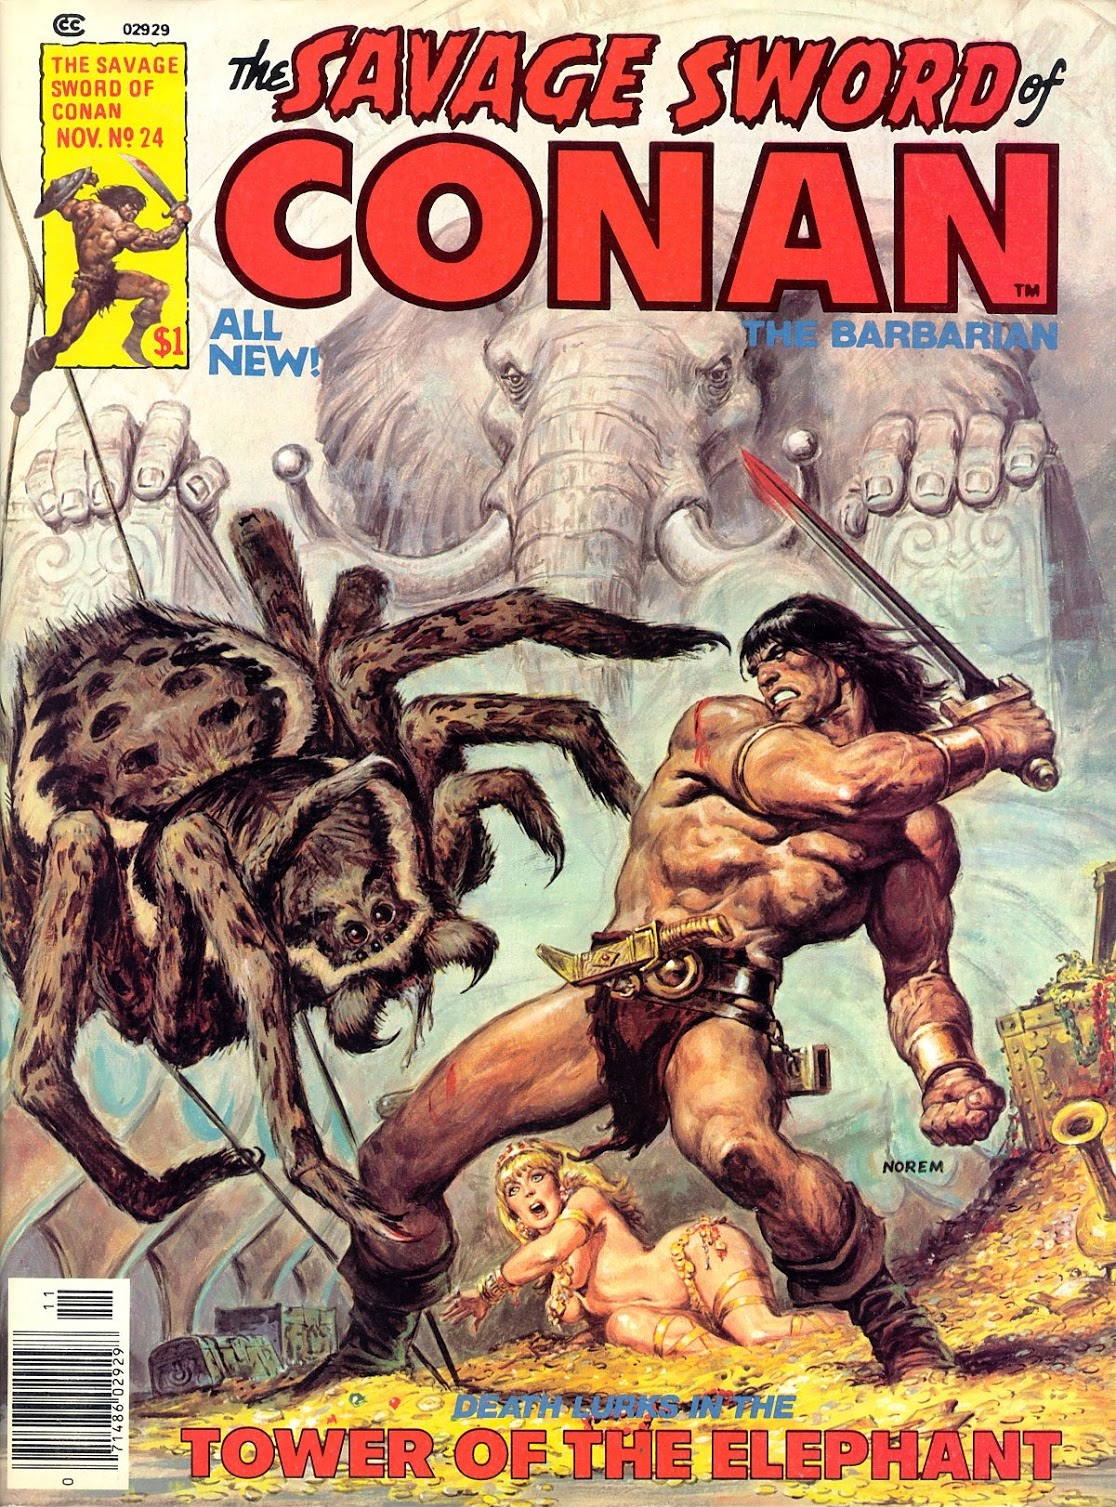
\includegraphics[width=0.6\textwidth]{img/TSSC24Portada}
        \caption{6 de Septiembre de 1977}
    \end{figure}
\column[t]{0.6\textwidth}
    \begin{itemize}
         \item Número 24 en la serie
         \item 65 páginas del ejemplar
         \item 40 de la historia
         \item Créditos:
         \begin{description}
            \item[Artista:] John Buscema
            \item[Artista:] Alfredo Alcalá
            \item[Escritor:] Roy Thomas
            \item[Portada:] Earl Norem
         \end{description}
    \end{itemize}
\end{columns}
\end{frame}
\note[itemize]{
	\item Este seria para mi el comic perfecto o el mas representativo de la edad de oro de Conan (ya se que tecnicament es la edad de bronze de los comics de lo 70 al 85)
	\item El Artista es John Buscema, es el hermano mayor de Sal Buscema. Tambien italoamericano, es para mi el mejor dibujante de Conan, de hecho, si a mi me piden que cierre los ojos y me imagine a Conan me lo imagino como lo dibujaba Jhon Buscema.
	\item El artista Filipino Alfredo Alcala es el segundo artista, probablemnet en la escenas de la narracion de YogKhosha. El ya habia hecho un personaje parecido a Conan, Voltar y se dice que Frank Frazetta se inspiro en el para hacer su propio Conan
	\item El artista norteamericano Earl Norem en la portada. Es probablemnete el artista que mas portadas de TSSC hizo durante la serie.
}

% \begin{frame}{}
% \begin{figure}[htp]
%  \centering
%  \begin{subfigure}[b]{0.16\textwidth}
%    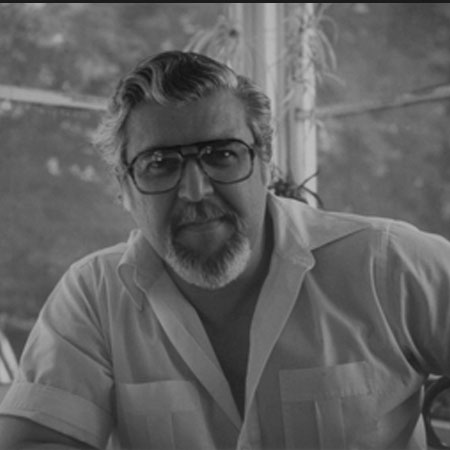
\includegraphics[width=\textwidth]{img/artistas/JohnBuscema}
%    \caption{John Buscema}
%  \end{subfigure}
% ~
%  \begin{subfigure}[b]{0.16\textwidth}
%    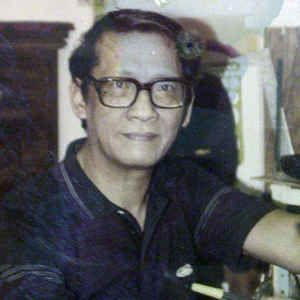
\includegraphics[width=\textwidth]{img/artistas/AlfredoAlcala}
%    \caption{Alfredo Alcalá}
%  \end{subfigure}
%  ~
%  \begin{subfigure}[b]{0.16\textwidth}
%    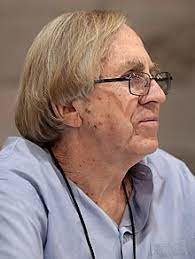
\includegraphics[width=\textwidth]{img/artistas/RoyThomas}
%    \caption{Roy Thomas}
%  \end{subfigure}
% ~
%  \begin{subfigure}[b]{0.16\textwidth}
%    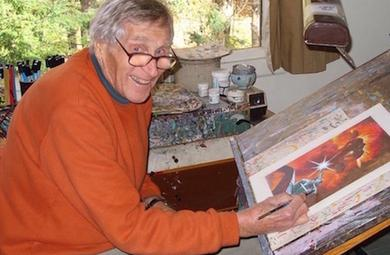
\includegraphics[width=\textwidth]{img/artistas/EarlNorem}
%    \caption{Earl Norem}
%  \end{subfigure}
% \end{figure}
% \end{frame}

\begin{frame}{Conan}
\begin{columns}
\column[t]{0.6\textwidth}
\begin{figure}[htp]
 \centering
 \begin{subfigure}[b]{0.3\textwidth}
   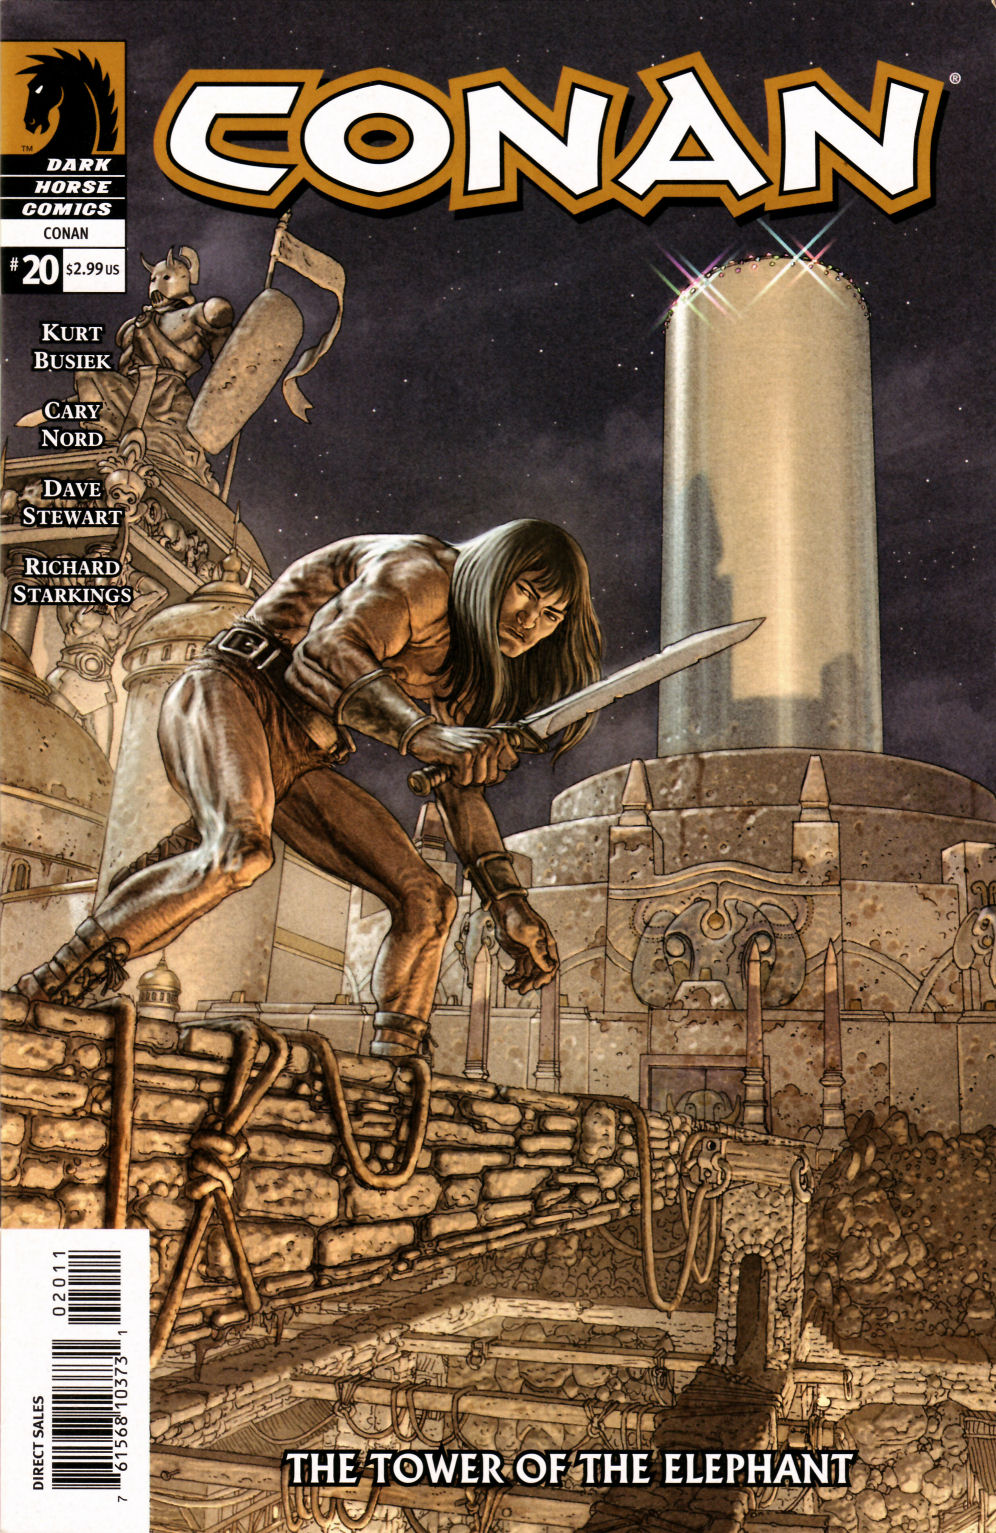
\includegraphics[width=\textwidth]{img/DarkHorse20Portada}
   \caption{Septiembre}
 \end{subfigure}
~
 \begin{subfigure}[b]{0.3\textwidth}
   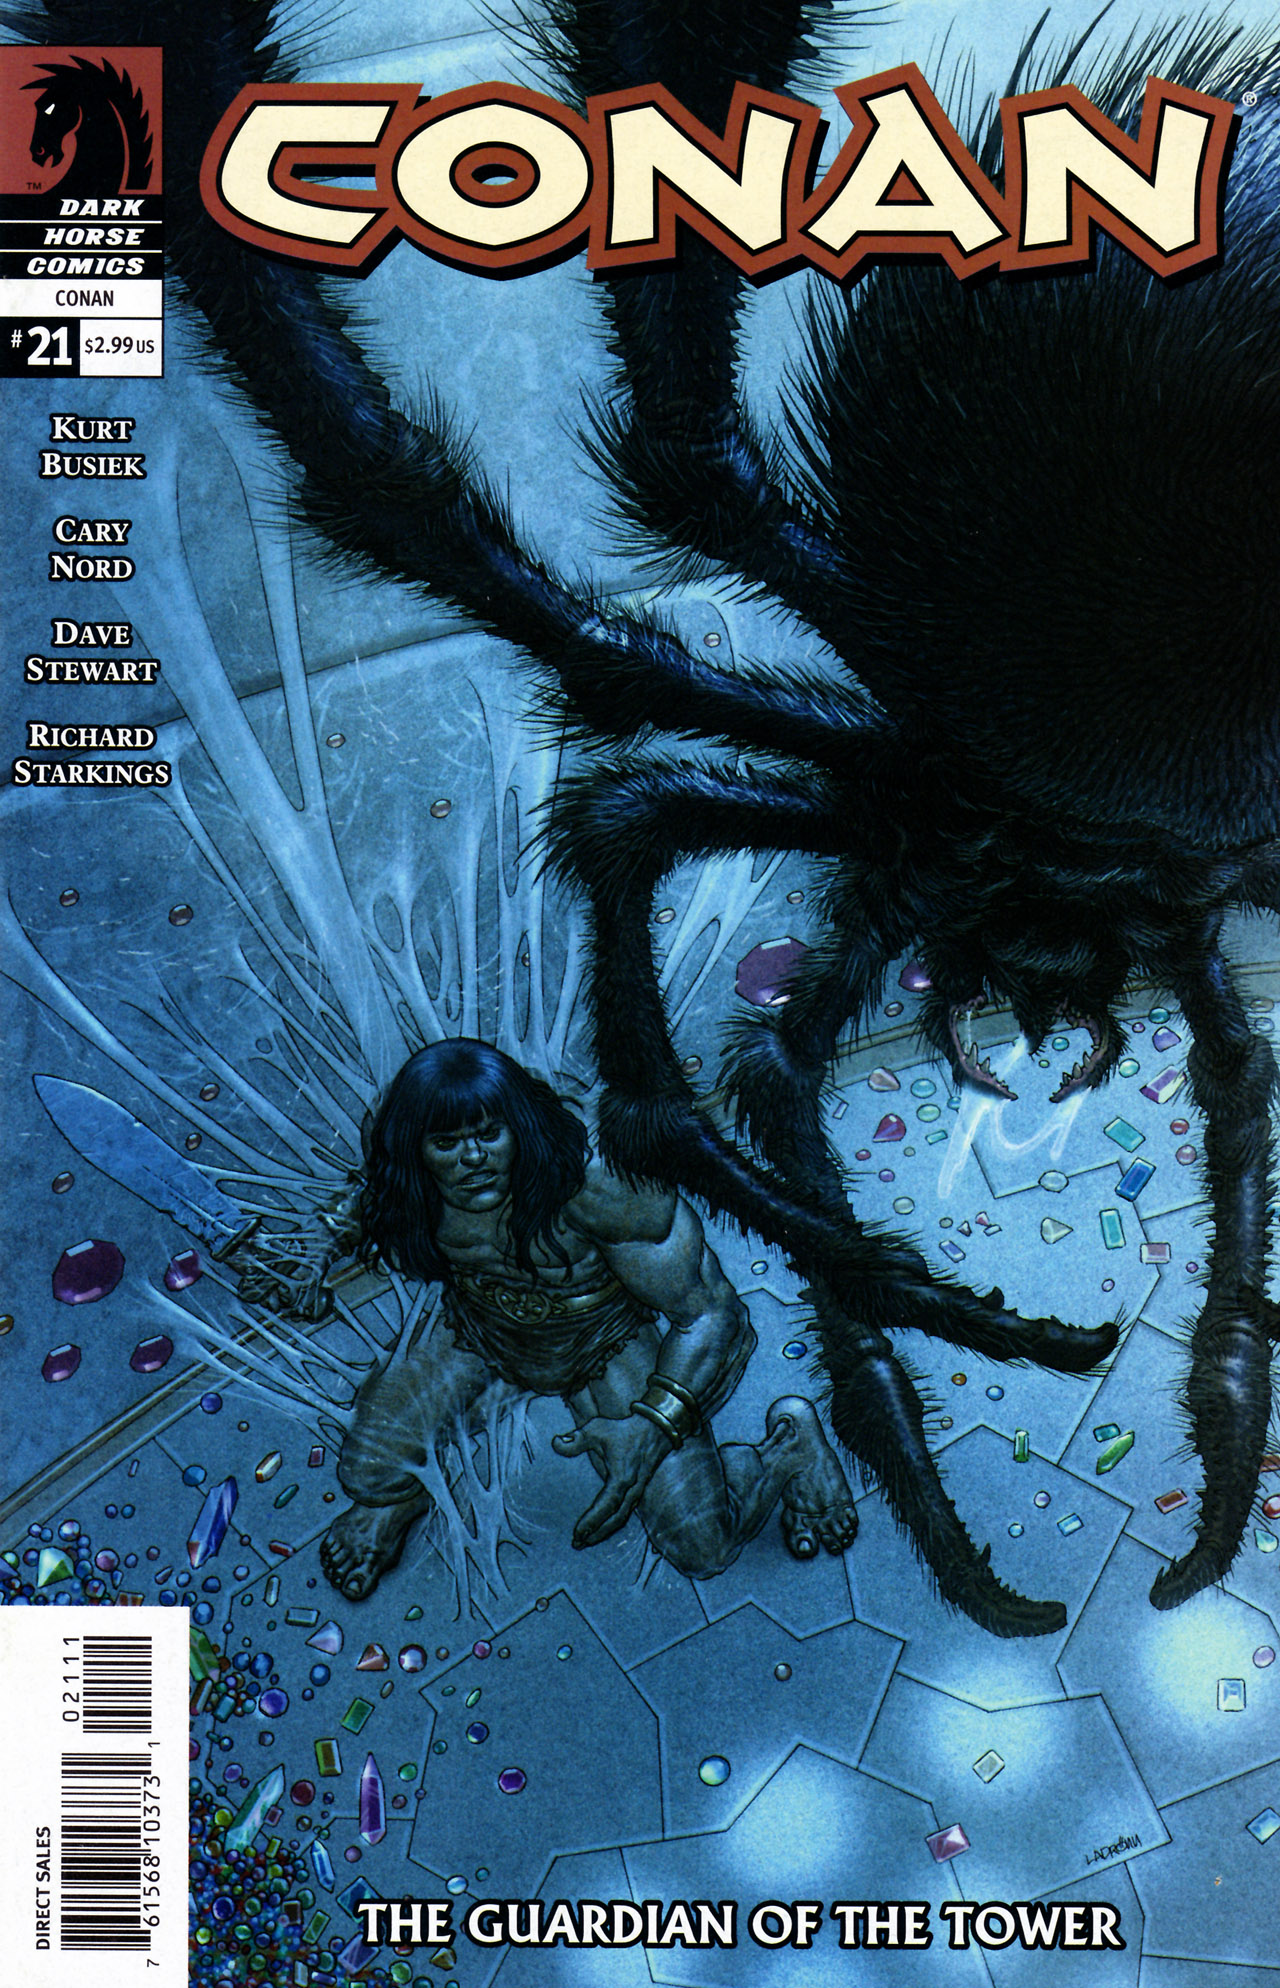
\includegraphics[width=\textwidth]{img/DarkHorse21Portada}
   \caption{Octubre}
 \end{subfigure}
 ~
 \begin{subfigure}[b]{0.3\textwidth}
   
\includegraphics[width=\textwidth]{img/DarkHorse22Portada}
   \caption{Noviembre}
 \end{subfigure}
\end{figure}
\begin{center}
2005
\end{center}
\column[t]{0.4\textwidth}
    \begin{itemize}
         \item \say{Conan de Dark Horse}
         \item Números 20, 21 y 22 en la serie
         \item 23, 25 y 26 pp. en cada ejemplar
         \item 20, 22 y 23 de la historia
         \item Créditos:
         \begin{description}
            \item[Artista:] Cary Nord
            \item[Artista(6pp):] Michael Kaluta
            \item[Escritor:] Kurt Busiek
            \item[Colorista:] Dave Steward
            \item[Portada:] José Ladrönn
            \item[Letrista:] Richard Starkings
         \end{description}
    \end{itemize}
\end{columns}
\end{frame}
\note[itemize]{
	\item Probablemnete la mejor adaptacion de la obra original de REH a un Comic.
	\i tem Uno de lo mejore miniarcos de Conan de DrakHrse, forma parte de su mejor volume el que simpremente se llamaba Conan
	\item Hereda parte del equiop creativo que ya habia ganado el Eisner por el numero 0
	\item Cuando vi por primera vez esta serie era una forma de hacer comics que nunca habia visto (sin entintador).Estos numeros tambien ocupan esa tecnica
	\item El canadiense Cary Nord en los trazos, que como dijimos gano el Eisner por el numero 0 de Conan, uno de los grandes dibujantes de Conan de todos los tiempos.
	\item Es escritor Estadounidense Kurt Busiek, el gran escritor de la corrida de Conan con DH, famoso por su comic Astro City, aqui hace una gran labor adaptando.
	\item El colorista estadounidense Dave Steward, que es una garantia, pues el solo tiene mas Eisners que todos los antes mencionados. Y que el pobre sufre la maldicion de los homonimos.
	\item El artista/pintor mexicano Jose Lardonn, oriundo de Veracruz, tambien con Eisner junto con Richard Stalking y que se ha dedicado mas al arte que a los comics. Este es uno de lo pocos ejemplos en las portadas. Kudos por la tercera portada
	\item El britanico Richard Starkings aka Comicraft, que es el mejor y mas famoso letrista en los comics hoy dia, famoso por elephanmen, y aun ligado a Conan con la mas reciente publicacion de Titan
}

\begin{frame}{Acción comics: La torre del elefante}
	\begin{columns}
		\column[t]{0.4\textwidth}
		\begin{figure}[htb]
			\centering
			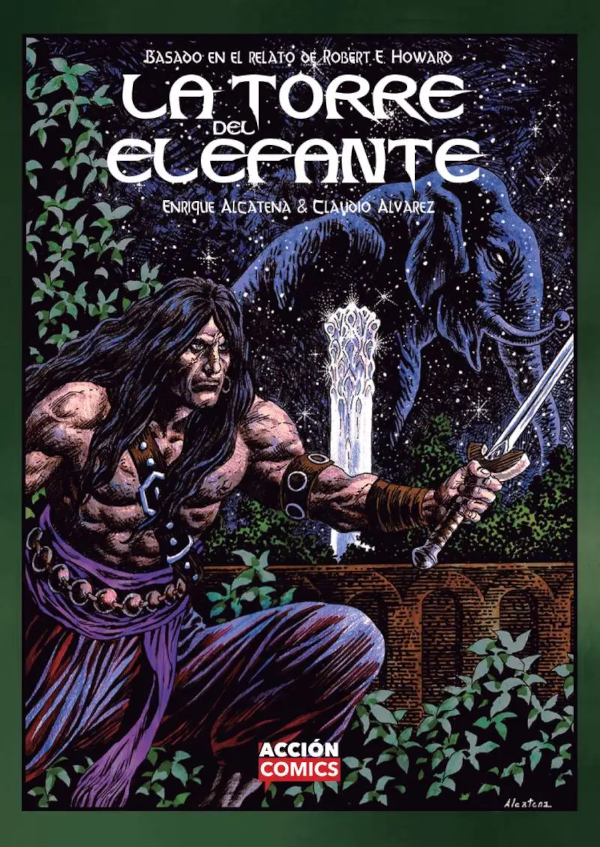
\includegraphics[width=0.6\textwidth]{img/AlcatenaTorre}
			\caption{Marzo 2025}
		\end{figure}
		\column[t]{0.6\textwidth}
		\begin{itemize}
			\item Tomo único
			\item Comic editado en Chile
			\item 76 páginas en Blanco y Negro
			\item Créditos:
			\begin{description}
				\item[Artista:] Enrique Alcatena
				\item[Escritor:] Claudio Álvarez
			\end{description}
			\begin{figure}[htb]
				\centering
				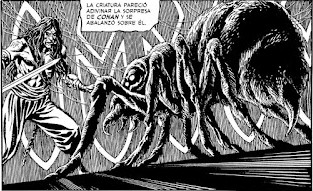
\includegraphics[width=0.4\textwidth]{img/AlcatenaTorre2}
			\end{figure}
		\end{itemize}
	\end{columns}
\end{frame}
\note[itemize]{
	\item Editorial Chilen Action Comics
	\item El artista argentino Enrique \say{Kike} alcatena, que ya antes habia dibujado a Conan para Marvel.
	\item El guionista y periodista Claudio Álvarez que forma parte de los fundadores de la editorial y que asumo que es Chileno.
}

\begin{frame}{Conan illustré: La Tour de l’Eléphant}
	\begin{columns}
		\column[t]{0.4\textwidth}
		\begin{figure}[htb]
			\centering
			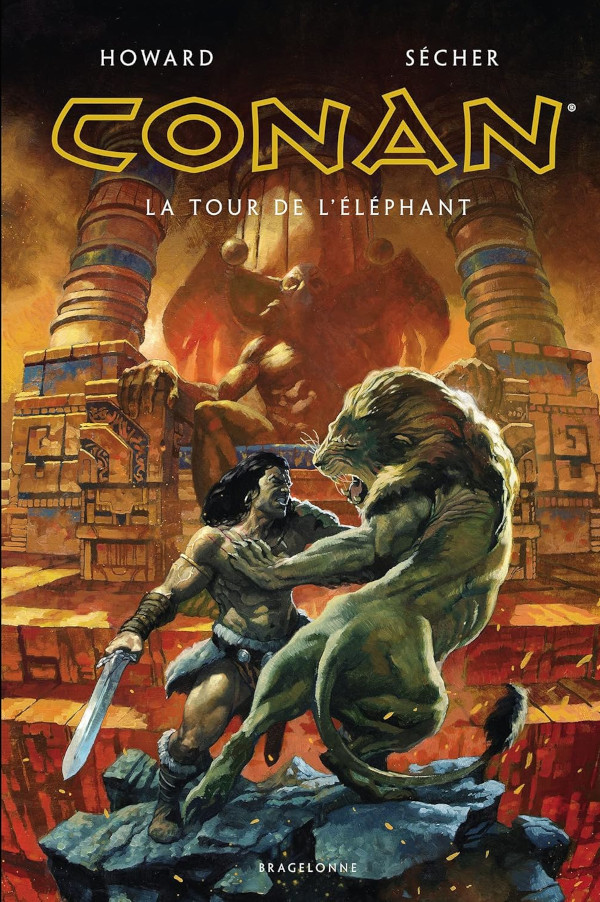
\includegraphics[width=0.6\textwidth]{img/SecherTorre}
			\caption{Octubre 2022}
		\end{figure}
		\column[t]{0.6\textwidth}
		\begin{itemize}
			\item No es una adaptación, es una edición ilustrada.
			\item Edición original en francés
			\item 56 páginas
			\item Créditos:
			\begin{description}
				\item[Artista:] Valentin Sécher
			\end{description}
		    \begin{figure}[htb]
			   \centering
			   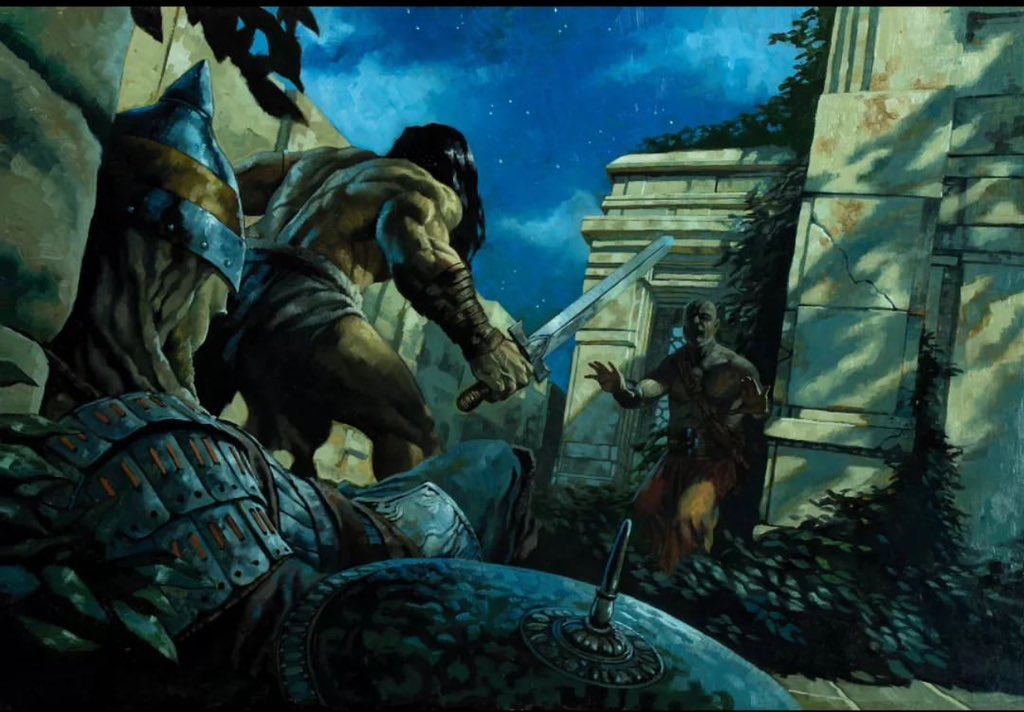
\includegraphics[width=0.45\textwidth]{img/vSecher}
     		\end{figure}
		\end{itemize}
	\end{columns}
\end{frame}
\note[itemize]{
	\item El ilustrado Frances Valentin Sécher, que ya antes habia hecho una obra de Conana ilustrada, pero ue es con esta l a que alacanza su prime.
	\item Es tan buena que la editorial Titan esta en platicas para hacer una edicion en Ingles (que se publicará en Agosto de este año)
}
% \begin{frame}{}
% \begin{figure}[htp]
%  \centering
%  \begin{subfigure}[b]{0.17\textwidth}
%    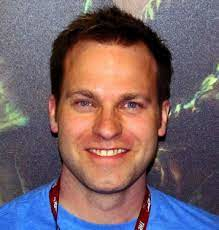
\includegraphics[width=\textwidth]{img/artistas/CaryNord}
%    \caption{Cary Nord}
%  \end{subfigure}
% ~
%  \begin{subfigure}[b]{0.17\textwidth}
%    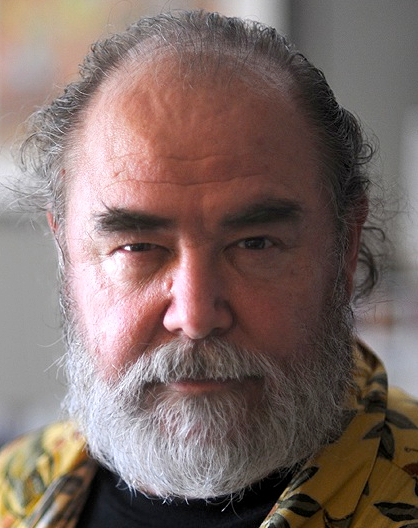
\includegraphics[width=\textwidth]{img/artistas/MichaelKaluta}
%    \caption{Michael Kaluta}
%  \end{subfigure}
% ~
%  \begin{subfigure}[b]{0.17\textwidth}
%    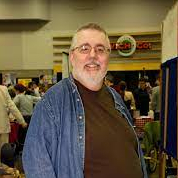
\includegraphics[width=\textwidth]{img/artistas/KurtBusiek}
%    \caption{Kurt Busiek}
%  \end{subfigure}
% \\
%  \begin{subfigure}[b]{0.17\textwidth}
%    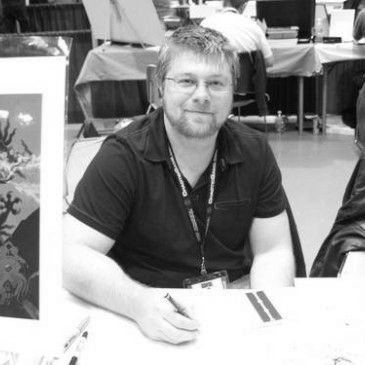
\includegraphics[width=\textwidth]{img/artistas/DaveStewart}
%    \caption{Dave Steward}
%  \end{subfigure}
% ~
%  \begin{subfigure}[b]{0.17\textwidth}
%    
\includegraphics[width=\textwidth]{img/artistas/JoseLadronn}
%    \caption{José Ladrönn}
%  \end{subfigure}
% ~
%  \begin{subfigure}[b]{0.17\textwidth}
%    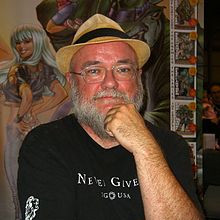
\includegraphics[width=\textwidth]{img/artistas/RichardStarkings}
%    \caption{Richard Starkings}
%  \end{subfigure}
% \end{figure}
% \end{frame}

\section{Resumen}
\note[itemize]{
	\item Toda la información anterior fue meramente monográfica.
	\item De aquí en adelante todo es un spoiler.
	\item Recomendar que se puede leer o escuchar la historia original en muchísimos lugares
	Voy a hacer un resumen usando viñetas de los antes mencionados comics
}

\begin{frame}{}
\begin{columns}
\column[t]{0.5\textwidth}
    \begin{figure}[htb]
    \centering
        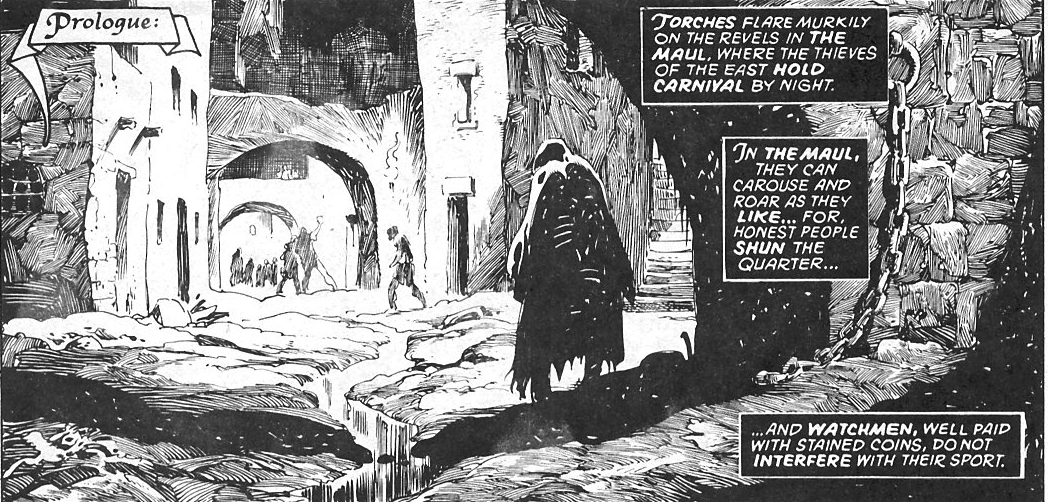
\includegraphics[width=0.9\textwidth]{img/res/01}
        \caption{El Maul}
    \end{figure}
\column[t]{0.5\textwidth}
    \begin{figure}[htb]
    \centering
        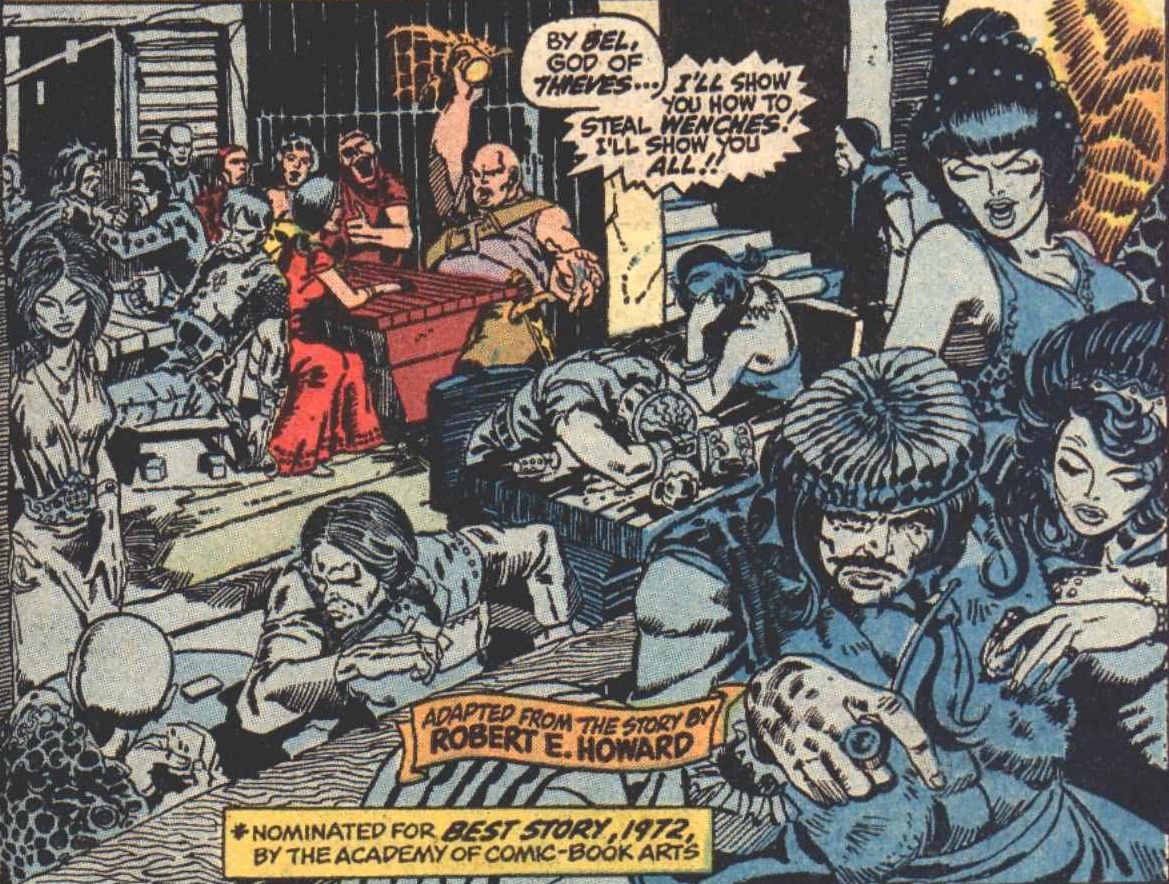
\includegraphics[width=0.9\textwidth]{img/res/02}
        \caption{Una taberna}
    \end{figure}
\end{columns}
\end{frame}
\note{
Todo el relato ocurre en una noche en la ciudad de Arenjunn, en la provincia de Zamora.
La historia comienza en una taberna del barrio del Maul.
La taberna está repleta de forajidos, ladrones, mercenarios, prostitutas y aventureros.
}

\begin{frame}{}
\begin{columns}
\column[t]{0.5\textwidth}
    \begin{figure}[htb]
    \centering
        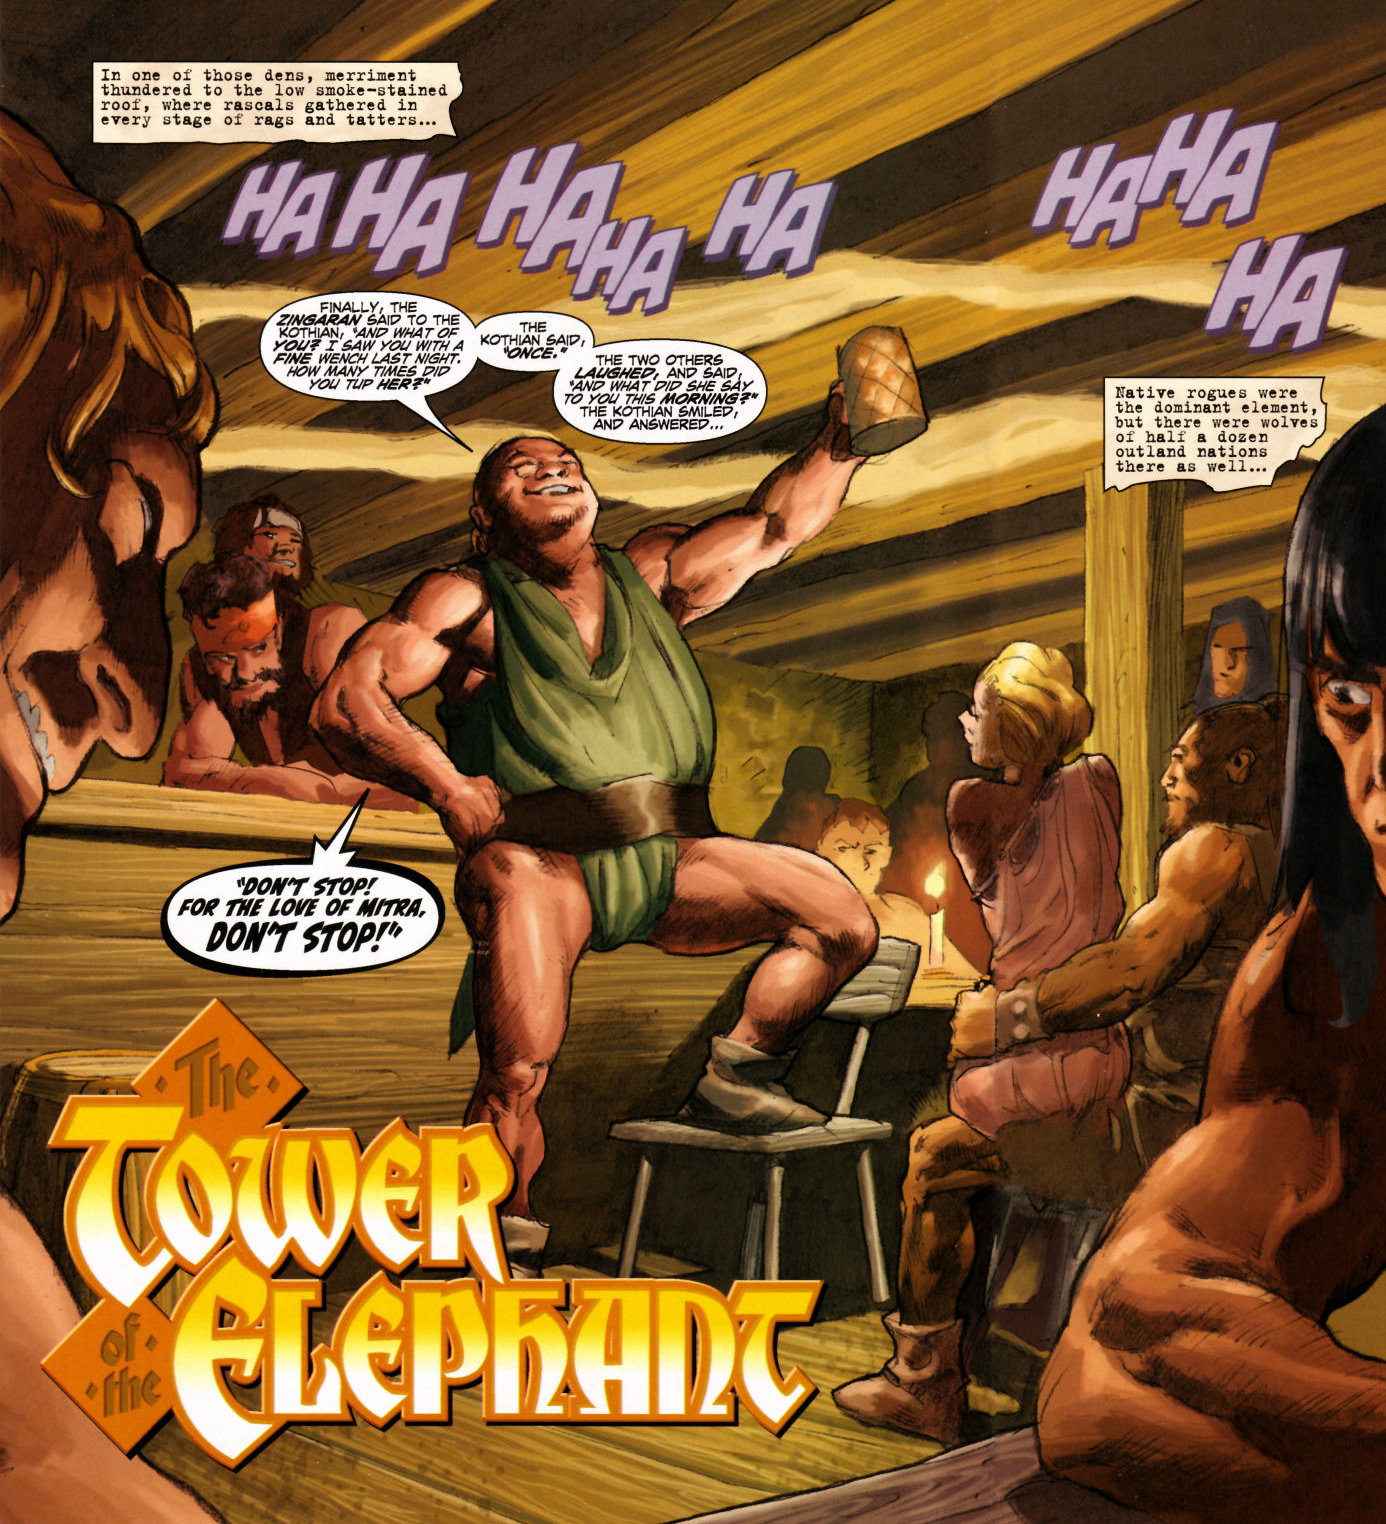
\includegraphics[width=0.65\textwidth]{img/res/03}
        \caption{El Kothio}
    \end{figure}
\column[t]{0.5\textwidth}
    \begin{figure}[htb]
    \centering
        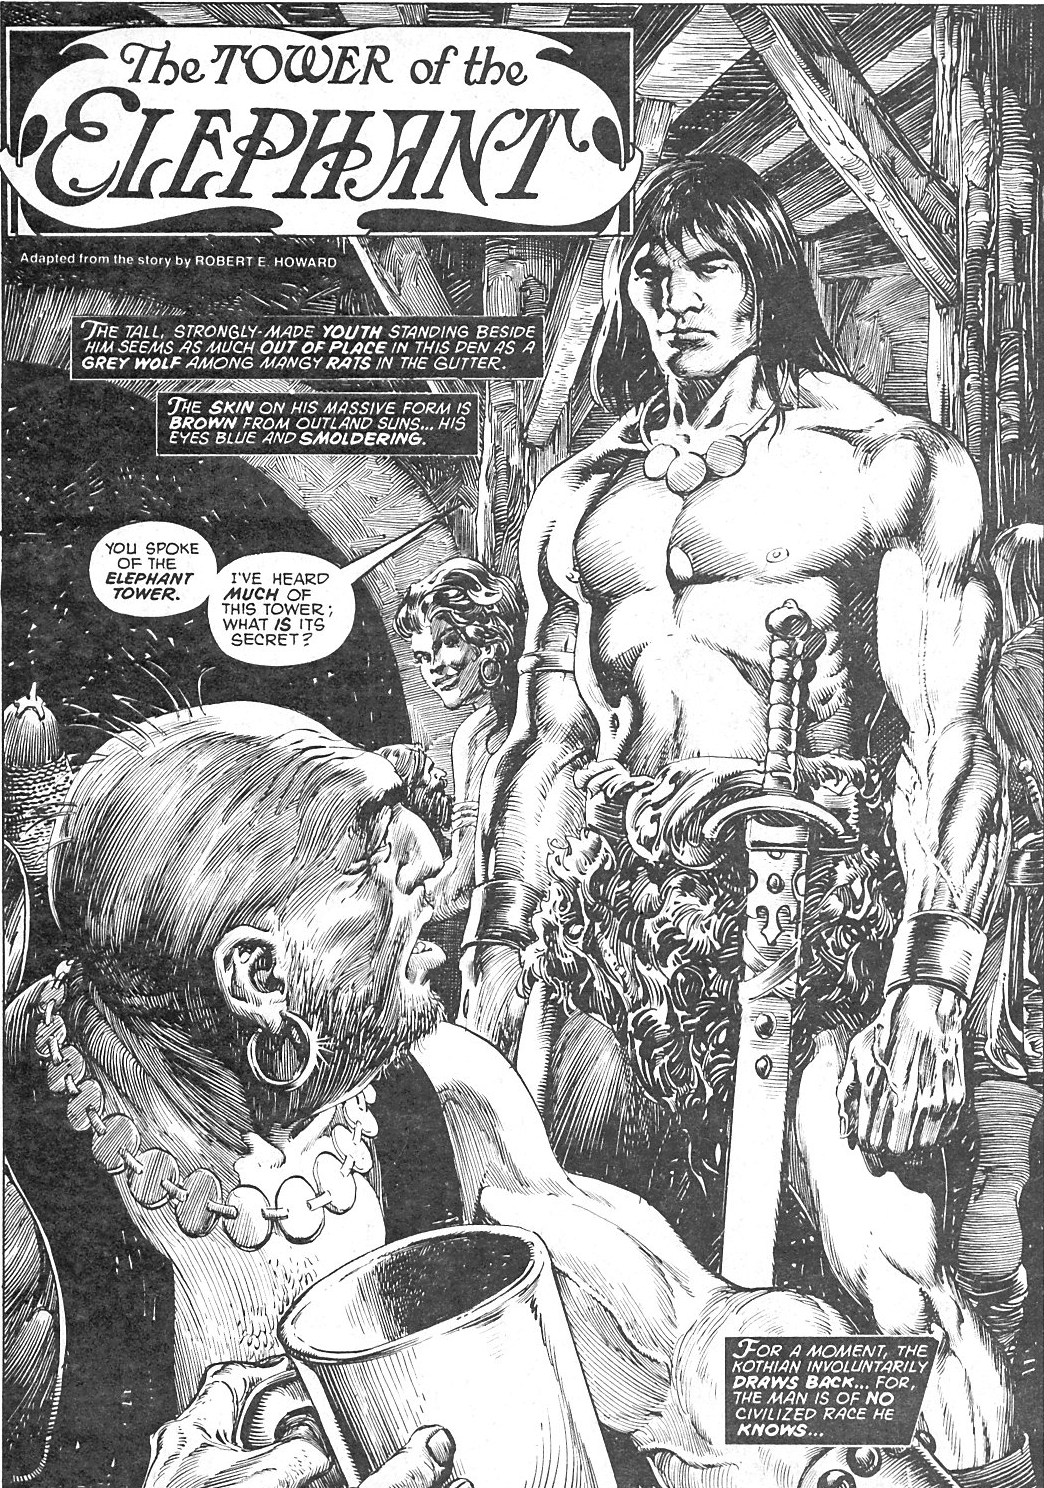
\includegraphics[width=0.55\textwidth]{img/res/04}
        \caption{Conan entra en escena}
    \end{figure}
\end{columns}
\end{frame}
\note{
Uno de ellos, está contando sus planes acerca de un crimen que planea cometer.
Mientras está narrando menciona la joya conocida como \say{el corazón del elefante} que está en posesión del temido hechicero Yara, en su torre.
Otro de los asistentes es Conan un bárbaro del norte; que en ese momento es muy joven --apenas ha dejado de ser un adolecente--.
}

\begin{frame}{}
\begin{columns}
\column[t]{0.5\textwidth}
    \begin{figure}[htb]
    \centering
        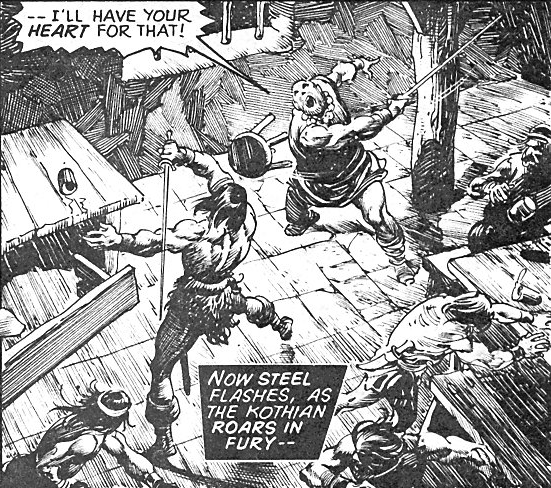
\includegraphics[width=0.7\textwidth]{img/res/05}
        \caption{Una pelea}
    \end{figure}
\column[t]{0.5\textwidth}
    \begin{figure}[htb]
    \centering
        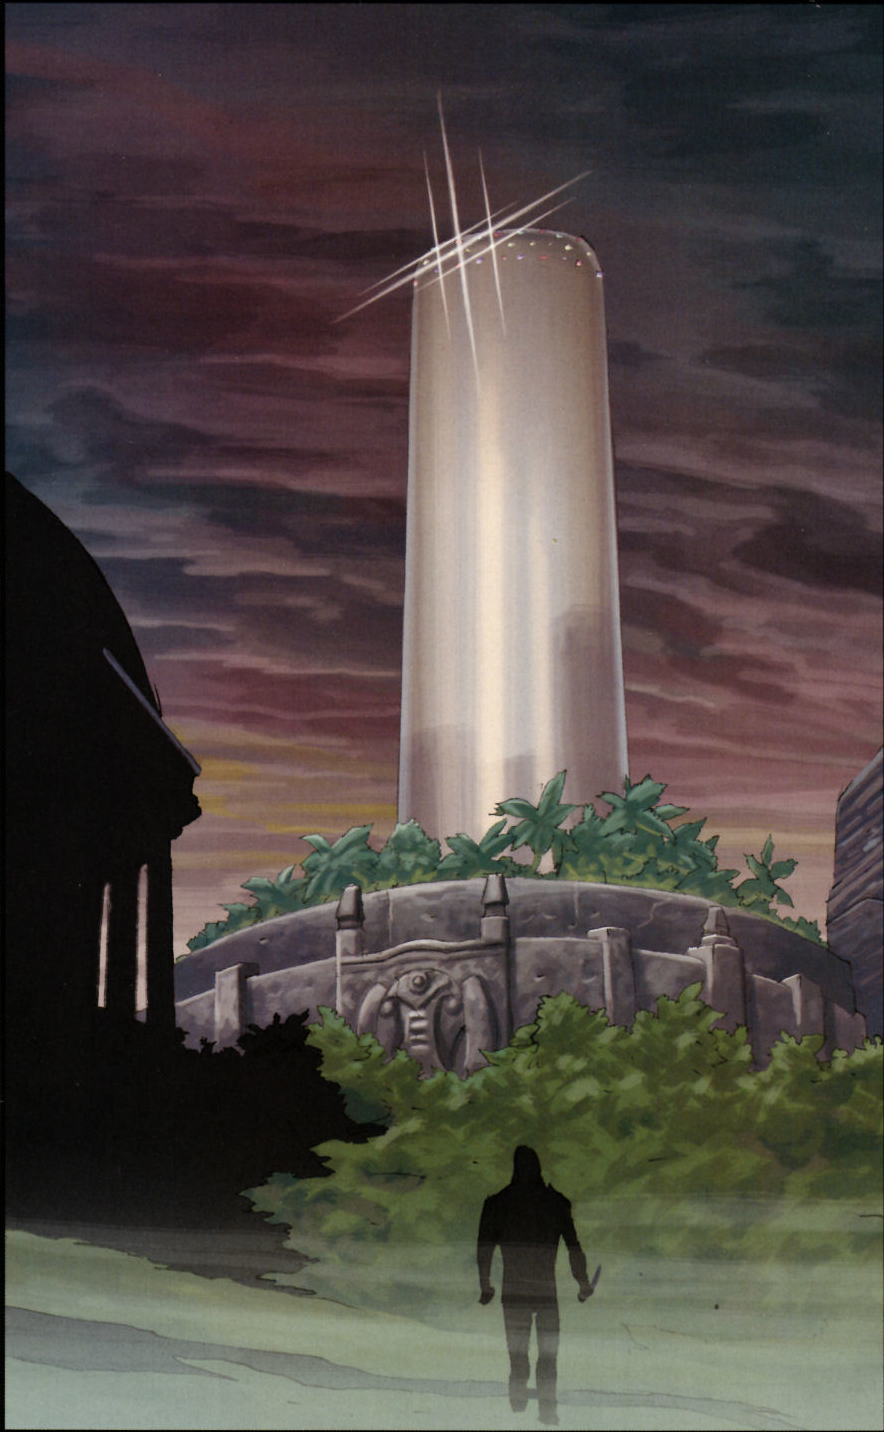
\includegraphics[width=0.4\textwidth]{img/res/06}
        \caption{La torre}
    \end{figure}
\end{columns}
\end{frame}
\note{
El bárbaro decide interrumpir la narración para preguntar con curiosidad acerca de la joya. Debido a la interrupción, empieza una discusión que termina en una pelea.
En medio de la confusión y después de matar a su oponente Conan escapa y decide encaminarse a \say{la torre del elefante} para tratar de robar la joya.
}

\begin{frame}{}
\begin{columns}
\column[t]{0.5\textwidth}
    \begin{figure}[htb]
    \centering
        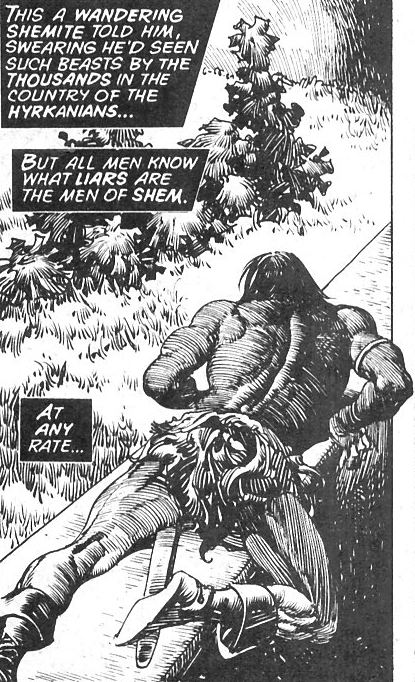
\includegraphics[width=0.5\textwidth]{img/res/07}
        \caption{El muro exterior}
    \end{figure}
\column[t]{0.5\textwidth}
    \begin{figure}[htb]
    \centering
        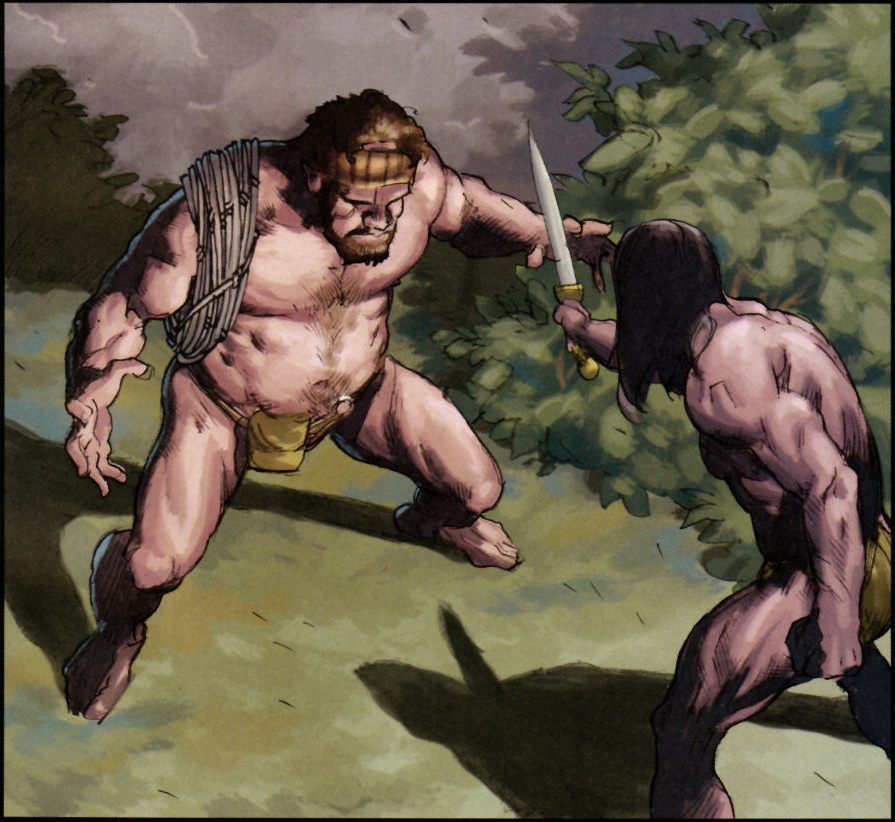
\includegraphics[width=0.7\textwidth]{img/res/08}
        \caption{Tauros de Nemedia}
    \end{figure}
\end{columns}
\end{frame}
\note{
Al llegar al edificio, se da cuenta de que los jardines inferiores de la torre están rodeados por un muro.
A falta de cualquier tipo de plan previo, Conan decide trepar el muro y matar al guardia que alcanza a oír del otro lado.
Sin embargo, al librar la barda y explorar dentro de los jardines, encuentra el cadáver del guardia y se da cuenta de que hay otra persona.

Sorprendentemente, en vez de atacarse mutuamente ambos hombres deciden hablar.
Conan se entera que su interlocutor es el famoso Tauros de Nemedia, conocido como \say{el príncipe de los ladrones}.
Y dado que ambos tienen el mismo objetivo y que Tauros se sorprende del arrojo de Conan proponen unir esfuerzos y compartir la aventura con el propósito de repartir el botín.
}

\begin{frame}{}
\begin{columns}
\column[t]{0.7\textwidth}
    \begin{figure}[htb]
    \centering
        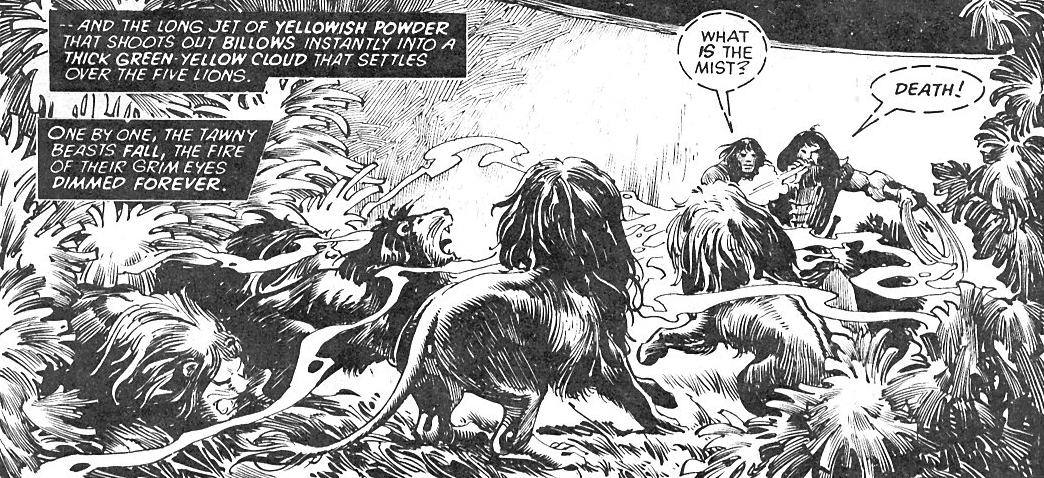
\includegraphics[width=0.85\textwidth]{img/res/09}
        \caption{Los guardianes del jardín}
    \end{figure}
\column[t]{0.3\textwidth}
    \begin{figure}[htb]
    \centering
        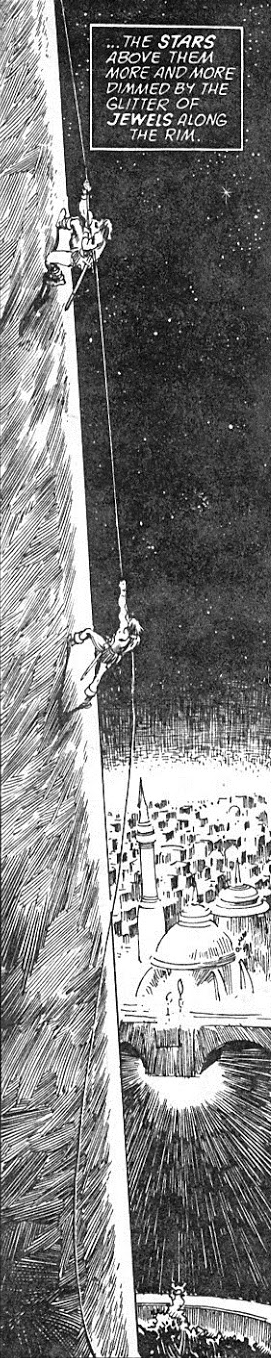
\includegraphics[width=0.28\textwidth]{img/res/10}
        \caption{Escalada}
    \end{figure}
\end{columns}
\end{frame}
\note{
Tauros advierte que en el jardín no hay guardias humanos, si no una jauría de leones. Pero también muestra estar preparado y con un artificio (gas envenenado) logran matar a los guardianes.

Al llegar al borde de la torre, deciden escalar por la pared exterior, dado que Tauros trae consigo una cuerda para tal propósito.
}

\begin{frame}{}
\begin{columns}
\column[t]{0.5\textwidth}
    \begin{figure}[htb]
    \centering
        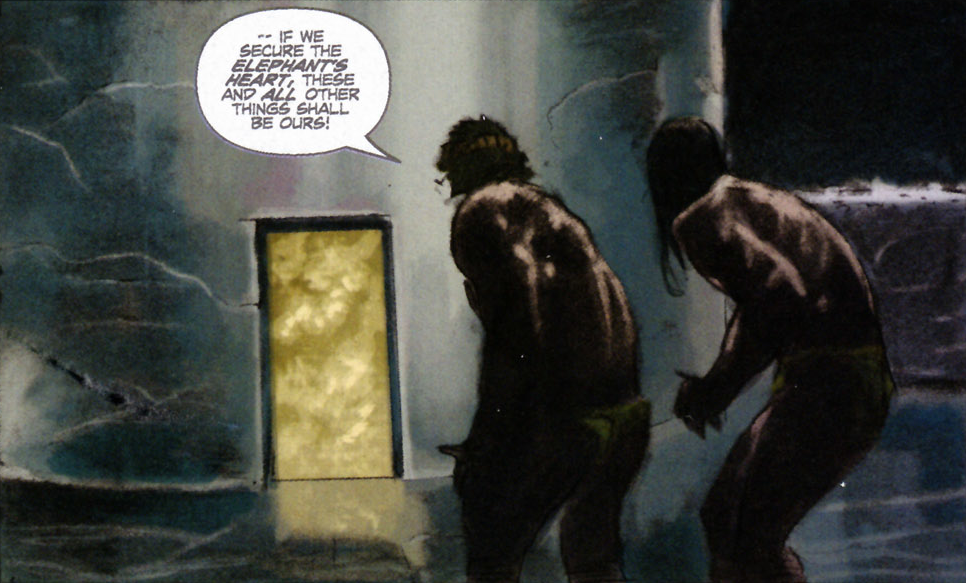
\includegraphics[width=0.8\textwidth]{img/res/11}
        \caption{Una puerta sin cerrojo}
    \end{figure}
\column[t]{0.5\textwidth}
    \begin{figure}[htb]
    \centering
        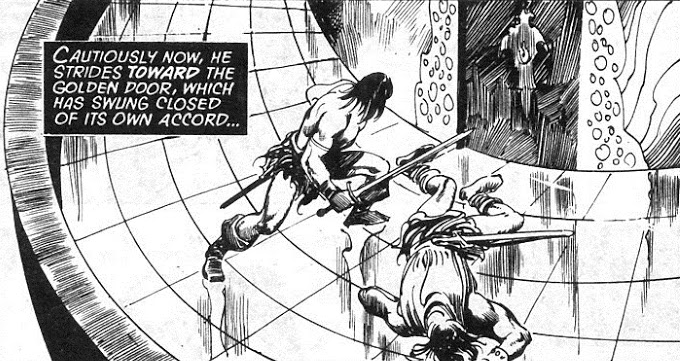
\includegraphics[width=0.9\textwidth]{img/res/12}
        \caption{El fin de Tauros}
    \end{figure}
\end{columns}
\end{frame}
\note{
Cuando alcanzan la azotea de la torre, se dan cuenta de que hay una puerta al interior que no está asegurada.
Tauros es el primero en entrar e instantes después sale por la misma puerta mortalmente herido y segundos después esta muerto.
}

\begin{frame}{}
\begin{columns}
\column[t]{0.4\textwidth}
    \begin{figure}[htb]
    \centering
        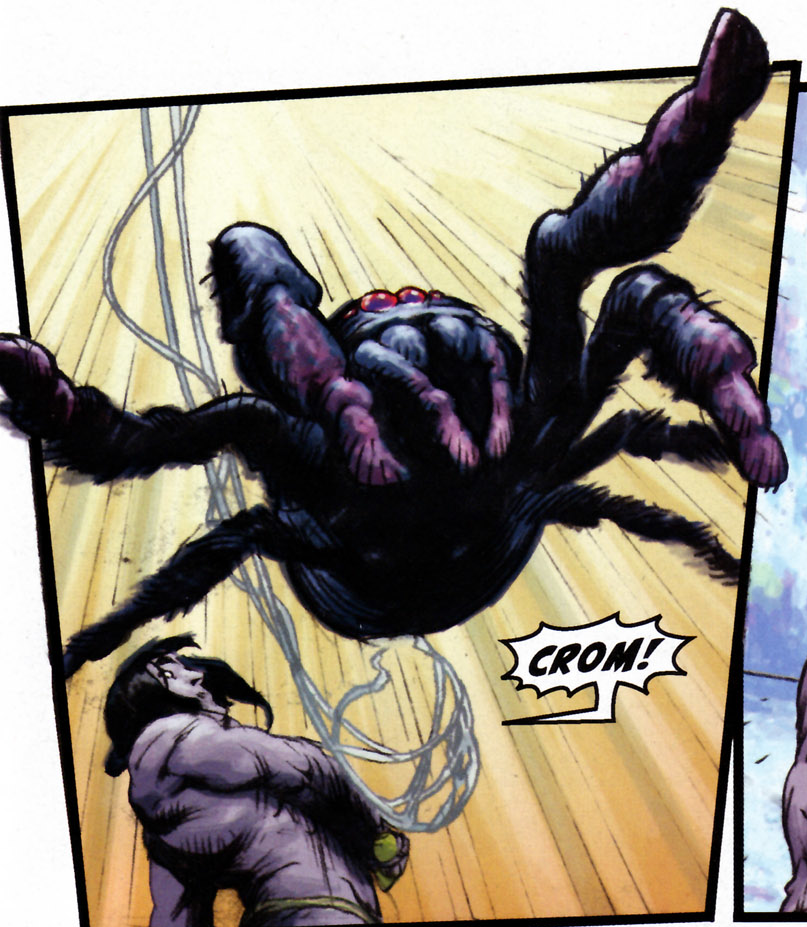
\includegraphics[width=0.7\textwidth]{img/res/13}
        \caption{El guardian de la torre}
    \end{figure}
\column[t]{0.6\textwidth}
    \begin{figure}[htb]
    \centering
        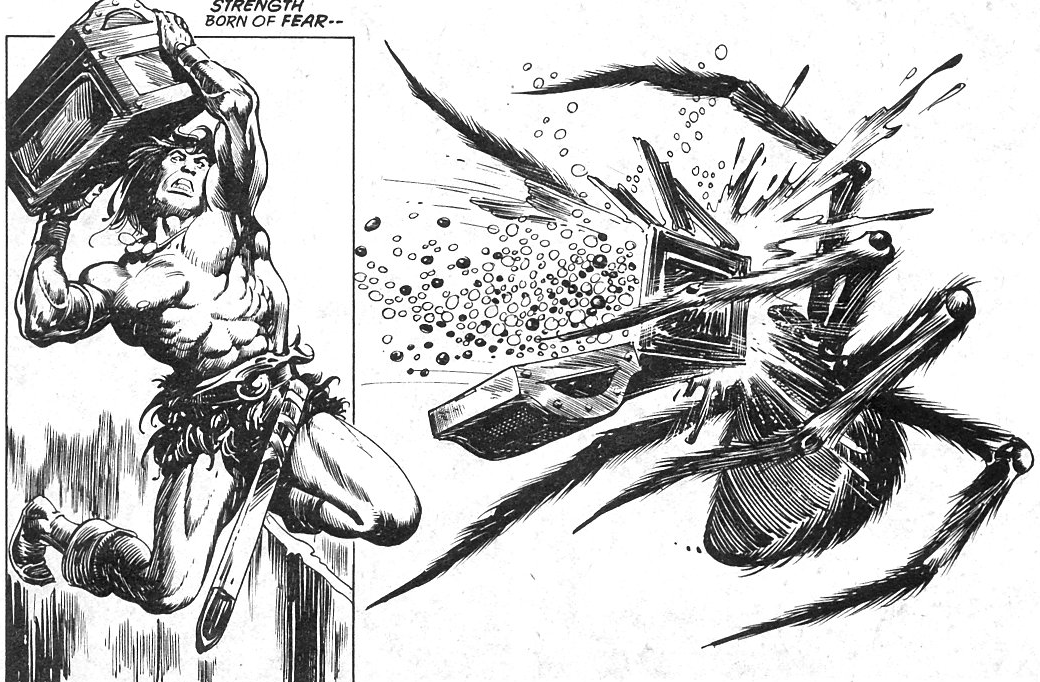
\includegraphics[width=0.85\textwidth]{img/res/14}
        \caption{Una muerte fortuita}
    \end{figure}
\end{columns}
\end{frame}
\note{
Conan decide terminar la aventura él solo, y al entrar por la puerta se ve obligado a confrontar al asesino de Tauros: una araña gigante.
Después de un intenso combate, Conan logra aplastar a la araña lanzandole un cofre y decide continuar su descenso por la torre.
}

\begin{frame}{}
\begin{columns}
\column[t]{0.6\textwidth}
    \begin{figure}[htb]
    \centering
        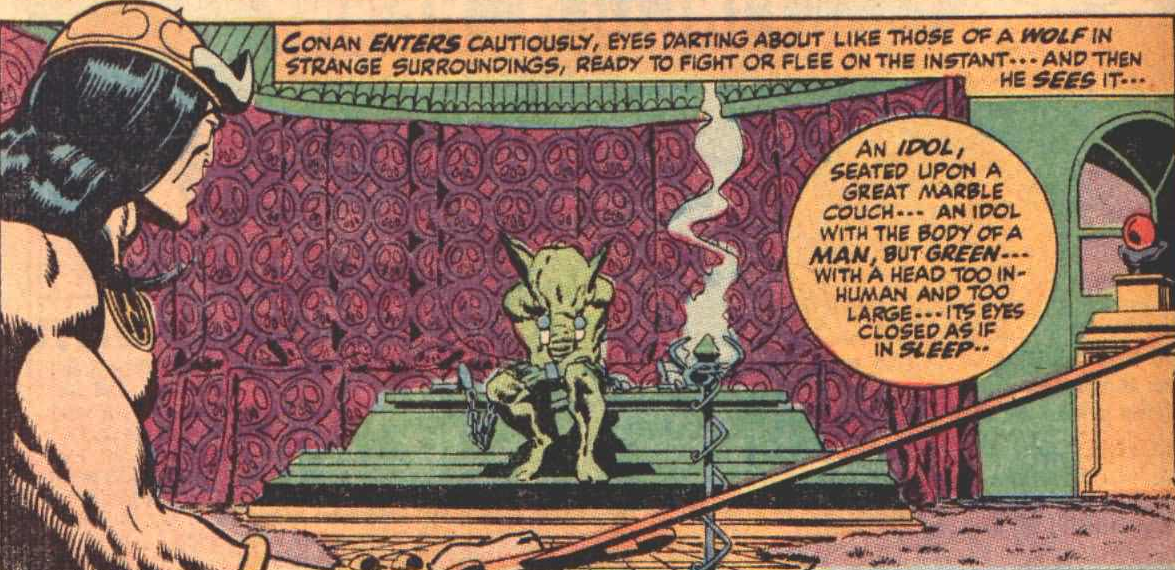
\includegraphics[width=0.85\textwidth]{img/res/15}
        \caption{El cautivo}
    \end{figure}
\column[t]{0.4\textwidth}
    \begin{figure}[htb]
    \centering
        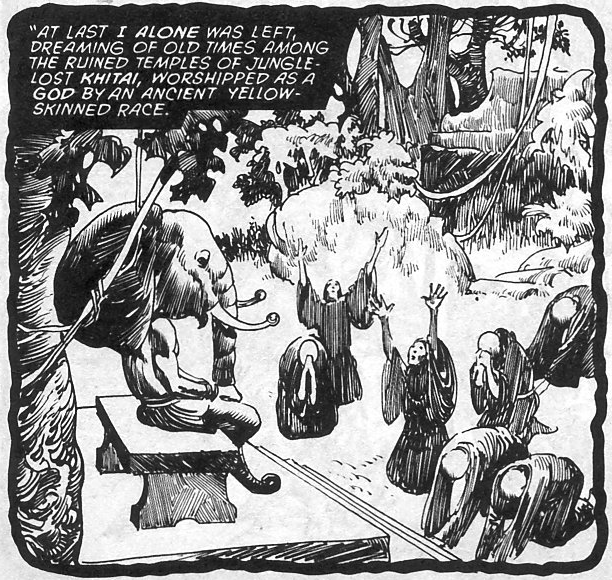
\includegraphics[width=0.85\textwidth]{img/res/16}
        \caption{Era venerado como un díos}
    \end{figure}
\end{columns}
\end{frame}
\note{
Conan llega a una cámara, en la que encuentra --lo que primero cree es-- un ídolo con cuerpo de hombre pero cabeza de elefante, pero después se da cuenta que es un ser viviente.

Al examinar más de cerca, se da cuenta de que el ser es un prisionero que ha sido torturado.
Cuando la presencia de Conan despierta al ser, éste le dice que su nombre es Yag-Khosa, y decide contarle su historia.

Yag-Khosa, es un ser de otro planeta que llegó a la tierra hace eones, junto con otros miembros de su especie.
Su raza posee conocimientos en las artes místicas y en las ciencias que superan por mucho a los de los humanos.
Al llegar a la tierra los seres elefantes, perdieron su capacidad de viajar entre los planetas y quedan atrapados en la tierra primitiva.
Cuando los humanos emergen en la tierra como la especie dominante, los seres elefantes se retiran a la selva de Kithai donde son adorados como dioses por los nativos.
Los seres van muriendo poco a poco hasta que Yag-Khosa, es el único sobreviviente de su raza.

En ese momento es cuando conoce a Yara un hombre que desea aprender de él los conocimientos místicos.
Yag-Khosa pasa años enseñando a Yara acerca de su magia.
Pero Yara, lleno de ambición; logra capturar y esclavizar a Yag-Khosa por medio de la traición.
Yag-Khosa describe como en los siglos que ha pasado en esclavitud, Yara lo ha obligado a cometer actos terribles por medio de tortura.
}

\begin{frame}{}
\begin{columns}
\column[t]{0.4\textwidth}
    \begin{figure}[htb]
    \centering
        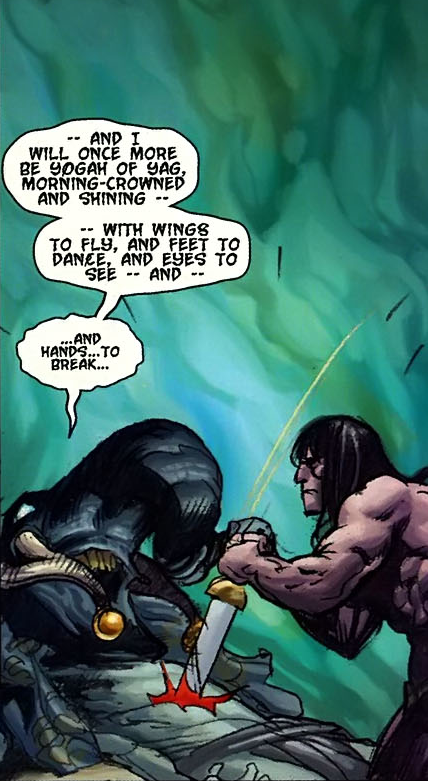
\includegraphics[width=0.55\textwidth]{img/res/17}
        \caption{Una muerte piadosa}
    \end{figure}
\column[t]{0.6\textwidth}
    \begin{figure}[htb]
    \centering
        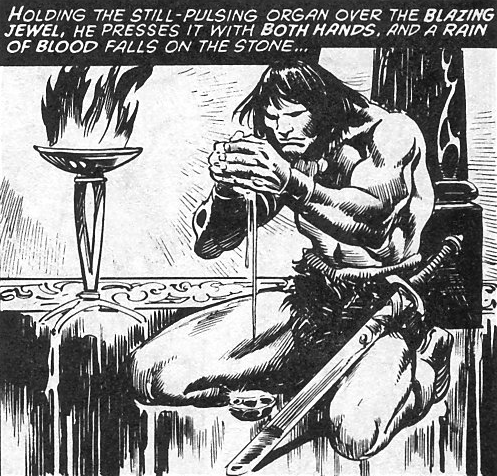
\includegraphics[width=0.7\textwidth]{img/res/18}
        \caption{El corazón y la sangre}
    \end{figure}
\end{columns}
\end{frame}
\note{
Después de terminar su narración, Yag-Khosa le pide a Conan que se apiade de él, lo mate y que siga unas instrucciones precisas que provocarán su venganza en contra  de Yara.
Yag-Khosa, le promete a Conan que si sigue sus instrucciones, él le dará a Conan una forma de salir a salvo de la torre.
Conan, accede, y tal como lo instruyó Yag-Khosa, entierra su espada en el pecho de la criatura, extrae su corazón y lo exprime vertiendo la sangre en en una joya (que entonces comprende es \say{El corazón del elefante}).
}

\begin{frame}{}
\begin{columns}
\column[t]{0.3\textwidth}
    \begin{figure}[htb]
    \centering
        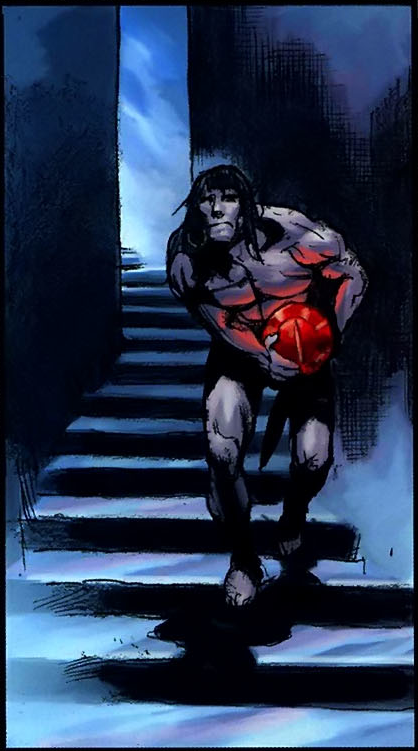
\includegraphics[width=0.7\textwidth]{img/res/19}
        \caption{Una promesa}
    \end{figure}
\column[t]{0.7\textwidth}
    \begin{figure}[htb]
    \centering
        \includegraphics[width=0.8\textwidth]{img/res/20}
        \caption{La venganza de Yag-Kosha}
    \end{figure}
\end{columns}
\end{frame}
\note{
Luego toma la joya y sale de la habitación.

Se dirige a un recinto inferior donde Yara, se encuentra meditando.
Cuando Conan entra a la habitación, Yara despierta y Conan --siguiendo las insturcciones--, le dice que este es un regalo de parte de Yag-Khosa y pone la joya enfrente de Yara.
}

\begin{frame}{}
\begin{columns}
\column[t]{0.5\textwidth}
    \begin{figure}[htb]
    \centering
        \includegraphics[width=0.8\textwidth]{img/res/21}
        \caption{El fin de Yaga}
    \end{figure}
\column[t]{0.5\textwidth}
    \begin{figure}[htb]
    \centering
        \includegraphics[width=0.5\textwidth]{img/res/22}
        \caption{La torre se derrumba}
    \end{figure}
\end{columns}
\end{frame}
\note{
Una especie de hechizo entra en efecto y Yara, se ve atraído hacia la joya mientras poco a poco va encogiéndose hasta que es un ser de unos cuantos centímetros que es absorbido por la joya.
Dentro de la joya el ser diminuto que ahora es Yara, es perseguido por una versión de Yag-Khosa que entendemos esta cumpliendo su venganza.

Despues de que  la venganza ha sido ejecutada, la torre empieza a derrumbarse y Conan logra salir sin encontrar ninguna resistencia.
Al parecer el resto de los guardianes han sido inhabilitados por la promesa de Yag-Khosa.

Finalmente, Conan logra salir de la torre y se pregunta si todo lo que paso ha sido un sueño. Pero al mirar hacia atrás observa el edificio, e instantes después éste se derrumba ante sus ojos.
}

\section{Personajes}
\note[itemize]{
	\item
}

\begin{frame}{Conan}
\begin{columns}
\column[t]{0.4\textwidth}
\begin{itemize}
 \item Un joven bárbaro del norte
 \item Intrépido, impulsivo y desconfiado
 \item Poco acostumbrado a la civilización
 \item Primitivo, fuerte y rebelde
\end{itemize}
\column[t]{0.6\textwidth}
\begin{figure}[htp]
 \centering
 \begin{subfigure}[b]{0.3\textwidth}
   \includegraphics[width=\textwidth]{img/conan/CTB}
 \end{subfigure}
~
 \begin{subfigure}[b]{0.27\textwidth}
   \includegraphics[width=\textwidth]{img/conan/DH}
 \end{subfigure}
~
 \begin{subfigure}[b]{0.23\textwidth}
   \includegraphics[width=\textwidth]{img/conan/TSSC}
 \end{subfigure}
\end{figure}
\end{columns}
\end{frame}
\note[itemize]{
	\item No olvidar que Conan representa varios arquetipos en sus diferentes aventuras.
	\item Esta al ser una de la primeras aventuras de su juventud predomina la idea del “salvaje noble”
}

\begin{frame}{Tauros}
\begin{columns}
\column[t]{0.4\textwidth}
\begin{itemize}
 \item Un ladrón de renombre
 \item Experimentado y arrogante
 \item Su apariencia engaña
 \item Astuto, preparado y lleno de recursos
\end{itemize}
\column[t]{0.6\textwidth}
\begin{figure}[htp]
 \centering
 \begin{subfigure}[b]{0.35\textwidth}
   \includegraphics[width=\textwidth]{img/tauros/TSSC}
 \end{subfigure}
~
 \begin{subfigure}[b]{0.3\textwidth}
   \includegraphics[width=\textwidth]{img/tauros/DH}
 \end{subfigure}
~
 \begin{subfigure}[b]{0.25\textwidth}
   \includegraphics[width=\textwidth]{img/tauros/CTB}
 \end{subfigure}
\end{figure}
\end{columns}
\end{frame}
\note[itemize]{
	\item
}

\begin{frame}{Yag-kosha}
\begin{columns}
\column[t]{0.4\textwidth}
\begin{itemize}
 \item Ser poderoso de otro  planeta, que ha sido esclavizado
 \item Viejo, sabio y derrotado
 \item Espera el momento de su venganza
 \item Busca la redención
 \item Referencia a el dios Hindu Ganesha
 \item Se autodenomina: Yogah de Yag, o Yog
\end{itemize}
\column[t]{0.6\textwidth}
\begin{figure}[htp]
 \centering
 \begin{subfigure}[b]{0.32\textwidth}
   \includegraphics[width=\textwidth]{img/yogh/CTB}
 \end{subfigure}
~
 \begin{subfigure}[b]{0.32\textwidth}
   \includegraphics[width=\textwidth]{img/yogh/DH}
 \end{subfigure}
\\
 \begin{subfigure}[b]{0.4\textwidth}
   \includegraphics[width=\textwidth]{img/yogh/TSSC}
 \end{subfigure}
\end{figure}
\end{columns}
\end{frame}
\note[itemize]{
	\item
}

\begin{frame}{Yara}
\begin{columns}
\column[t]{0.4\textwidth}
\begin{itemize}
 \item Hechicero poderoso y malvado
 \item Cruel, traicionero y ambicioso
 \item Arrogante, no teme perder su poder
\end{itemize}
\column[t]{0.6\textwidth}
\begin{figure}[htp]
 \centering
 \begin{subfigure}[b]{0.25\textwidth}
   \includegraphics[width=\textwidth]{img/yara/TSSC}
 \end{subfigure}
~
 \begin{subfigure}[b]{0.2\textwidth}
   \includegraphics[width=\textwidth]{img/yara/DH}
 \end{subfigure}
~
 \begin{subfigure}[b]{0.2\textwidth}
   \includegraphics[width=\textwidth]{img/yara/CTB}
 \end{subfigure}
\end{figure}
\end{columns}
\end{frame}
\note[itemize]{
	\item
}

\begin{frame}{Kothio anónimo}
\begin{columns}
\column[t]{0.4\textwidth}
\begin{itemize}
 \item Un criminal de poca monta
 \item Alardea de proezas por llevar a cabo
 \item Descortés y confiado
\end{itemize}
\column[t]{0.6\textwidth}
\begin{figure}[htp]
 \centering
 \begin{subfigure}[b]{0.3\textwidth}
   \includegraphics[width=\textwidth]{img/khotio/TSSC}
 \end{subfigure}
~
 \begin{subfigure}[b]{0.25\textwidth}
   \includegraphics[width=\textwidth]{img/khotio/DH}
 \end{subfigure}
~
 \begin{subfigure}[b]{0.25\textwidth}
   \includegraphics[width=\textwidth]{img/khotio/CTB}
 \end{subfigure}
\end{figure}
\end{columns}
\end{frame}
\note[itemize]{
	\item
}

\begin{frame}{La torre del elefante}
\begin{columns}
\column[t]{0.4\textwidth}
\begin{itemize}
 \item Edificio-fortaleza que domina la ciudad
 \item Edificado por medio de magia
\end{itemize}
\column[t]{0.6\textwidth}
\begin{figure}[htp]
 \centering
 \begin{subfigure}[b]{0.5\textwidth}
   \includegraphics[width=\textwidth]{img/torre/TSSC}
 \end{subfigure}
~
 \begin{subfigure}[b]{0.08\textwidth}
   \includegraphics[width=\textwidth]{img/torre/DH}
 \end{subfigure}
~
 \begin{subfigure}[b]{0.1\textwidth}
   \includegraphics[width=\textwidth]{img/torre/CTB}
 \end{subfigure}
\end{figure}
\end{columns}
\end{frame}
\note[itemize]{
	\item
}

\begin{frame}{Araña gigante}
\begin{columns}
\column[t]{0.4\textwidth}
\begin{itemize}
 \item Guardián del piso superior de la torre
 \item Astuto, pese a ser una bestia
\end{itemize}
\column[t]{0.6\textwidth}
\begin{figure}[htp]
 \centering
 \begin{subfigure}[b]{0.5\textwidth}
   \includegraphics[width=\textwidth]{img/arana/TSSC}
 \end{subfigure}
\\
 \begin{subfigure}[b]{0.3\textwidth}
   \includegraphics[width=\textwidth]{img/arana/DH}
 \end{subfigure}
~
 \begin{subfigure}[b]{0.2\textwidth}
   \includegraphics[width=\textwidth]{img/arana/CTB}
 \end{subfigure}
\end{figure}
\end{columns}
\end{frame}
\note[itemize]{
	\item No olvidemos que el libro de Tolkien fue publicado en el 54.
}

\begin{frame}{Los leones}
\begin{columns}
\column[t]{0.4\textwidth}
\begin{itemize}
 \item Guardianes del jardín interior
 \item Simbolizan la fuerza primitiva
 \item Algunas cualidades sobrenaturales
 \item Sucumben ante el polvo mortal
 \item Uno de ellos casi logra su venganza
\end{itemize}
\column[t]{0.6\textwidth}
\begin{figure}[htp]
 \centering
 \begin{subfigure}[b]{0.4\textwidth}
   \includegraphics[width=\textwidth]{img/leones/TSSC}
 \end{subfigure}
~
 \begin{subfigure}[b]{0.3\textwidth}
   \includegraphics[width=\textwidth]{img/leones/DH}
 \end{subfigure}
\\
\vspace{0.5cm}
 \begin{subfigure}[b]{0.6\textwidth}
   \includegraphics[width=\textwidth]{img/leones/CTB}
 \end{subfigure}
\end{figure}
\end{columns}
\end{frame}
\note[itemize]{
	\item  Howard siempre profirió en sus historias profunda admiración por los felinos.
	\item De hecho siempre que describe a sus protagonistas, no solo en el ciclo de Conan sino en todas sus obras, les da cualidades que son comparables a las de algún felino.
}


\section{Citas interesantes}
\note[itemize]{
	\item Poder comparar la prosa económica de Howard en ambos idiomas.
	\item Tanto para ver que tanta justicia hay en la traducción.
	\item Recordemos que Howard era poeta y que su lírica se asoma aun en su prosa, que es lo que lo hace excepcional como escritor de Pulp, el efecto de drama
}

\begin{frame}{Conan reflexiona sobre religión}
\begin{exampleblock}{}
He had squatted for hours in the courtyard of the philosophers, listening to the arguments of theologians and teachers, and come away in a haze of bewilderment, sure of only one thing, and that, that they were all touched in the head.
\end{exampleblock}

\begin{itemize}
	\item \textit{ \say{Había estado muchas horas en cuclillas en los patios de los filósofos, escuchando los razonamientos y discusiones de teólogos y maestros, y se había ido de allí confuso y perplejo y con una sola idea clara: que estaban todos locos.} }
\end{itemize}
\end{frame}
\note[itemize]{
	\item  Esta es una cita que describe mucho de la personalidad de Conan en su edad temprana y que es paradigmática de cómo el personaje evoluciona porque en el Fénix en la espada tiene una opinión muy diferente (y esa historia fue de hecho escrita antes)
}

\begin{frame}{Hombres civilizados discutiendo}

\begin{exampleblock}{}
Civilized men are more discourteous than savages because they know they can be impolite without having their skulls split, as a general thing.
\end{exampleblock}

\begin{itemize}
	\item \textit{ \say{Los hombres civilizados son menos amables que los salvajes porque saben que pueden ser descorteses sin correr el riesgo de que les partan la cabeza; por regla general.} }
\end{itemize}

\end{frame}
\note[itemize]{
	\item Una de las citas más famosas de Howard (ocurre en este relato). Este es Howard en su sentir más íntimo.
}

\begin{frame}{La culpabilidad de una raza sobre sus hombros}
\begin{exampleblock}{}
	And suddenly all fear and repulsion went from him, to be replaced by a great pity. What this monster was, Conan could not know, but the evidences of its sufferings were so terrible and pathetic that a strange aching sadness came over the Cimmerian, he knew not why. He only felt that he was looking upon a cosmic tragedy, and he shrank with shame, as if the guilt of a whole race were laid upon him.
\end{exampleblock}

\begin{itemize}
	\item \textit{ \say{Y súbitamente todo el miedo y el asco se convirtieron en una profunda compasión. Conan no sabía quién era ese monstruo, pero era tan evidente su terrible y patético sufrimiento, que sin saber por qué, le embargó una abrumadora tristeza. Sintió que estaba presenciando una tragedia cósmica y sintió vergüenza, como si la culpa de toda una raza hubiera caído sobre él.} }
\end{itemize}

\end{frame}
\note[itemize]{
	\item Mi cita favorita del relato.
}

\section{Tropes literarios}
\note[itemize]{
	\item
}

\begin{frame}{Espada y hechizeria}
\begin{columns}
\column[t]{0.4\textwidth}
 \begin{itemize}
    \item Temporalidad: una sola noche
    \item Aventura circunstancial
    \item No genero un cambio
    \item La espada: la justicia; la hechicería: el mal
 \end{itemize}
 \column[t]{0.6\textwidth}
 \begin{figure}[htb]
    \centering
    \includegraphics[width=0.8\textwidth]{img/tributos/elephant07}
    \caption{Abe Papakhian}
 \end{figure}
 \end{columns}
\end{frame}
\note[itemize]{
	\item
}

\begin{frame}{Taberna}
	\begin{columns}
		\column[t]{0.4\textwidth}
		\begin{itemize}
			\item En la taberna del pueblo se congregan todos los maleantes
			\item Altas probabilidades de una pelea
			\item Los agentes de la ley no intervienen, o llegaran tarde
		\end{itemize}
		\column[t]{0.6\textwidth}
		\begin{figure}[htb]
			\centering
			\includegraphics[width=0.7\textwidth]{img/tropes/taberna}
		\end{figure}
	\end{columns}
\end{frame}
\note[itemize]{
	\item
}

\begin{frame}{Conan el ladrón, el antihéroe}
\begin{columns}
\column[t]{0.4\textwidth}
 \begin{itemize}
   \item Busca su beneficio personal
   \item Es el instrumento de la justicia, solo por que lo arrojan las circunstancias
   \item Se adhiere a su propio código de ética: simple y primitivo
 \end{itemize}
 \column[t]{0.6\textwidth}
 \begin{figure}[htb]
    \centering
    \includegraphics[width=0.25\textwidth]{img/tropes/antiheroe}
 \end{figure}
 \end{columns}
\end{frame}
\note[itemize]{
	\item Recordemos que Conan tiene distintos estereotipos a lo largo de sus aventuras.
	\item En esta etapa Conan no es un héroe, no sigue el camino del héroe como diría Joseph Campbell.
	\item Aunque bueno en los análisis que revise, hay uno donde lo hacen entrar con calzador. Esto no es cierto en esta historia Conan es un antihéroe.
}

\begin{frame}{Instintos superan la razón}
\begin{columns}
\column[t]{0.4\textwidth}
 \begin{itemize}
    \item Al escapar del león
    \item Y luego de la araña
    \item No se vuelve loco al ver a Yag-kosha
    \item Conan crítica los eruditos y triunfa por sus instintos
 \end{itemize}
 \column[t]{0.6\textwidth}
 \begin{figure}[htb]
    \centering
    \includegraphics[width=0.6\textwidth]{img/tropes/instintos}
 \end{figure}
 \end{columns}
\end{frame}
\note[itemize]{
	\item
}

\begin{frame}{Conan odia y teme lo sobrenatural}
\begin{columns}
\column[t]{0.4\textwidth}
 \begin{itemize}
    \item Se asusta con:
    \begin{itemize}
      \item La magia en general
      \item La historia que se cuenta de Yara
      \item El polvo que mata a lo leones
      \item La araña gigante
      \item Al ver a Yag-kosha
    \end{itemize}
 \end{itemize}
 \column[t]{0.6\textwidth}
 \begin{figure}[htb]
    \centering
    \includegraphics[width=0.3\textwidth]{img/tropes/temor}
 \end{figure}
 \end{columns}
\end{frame}
\note[itemize]{
	\item Conan no teme a ningún ser humano y menos a la muerte en batalla. Sin embargo, se puede paralizar de terror ante la magia o lo sobrenatural.
	\item De nuevo en esta etapa de su carrera.
}

\begin{frame}{Los cimerios escalando}
  \begin{columns}
  \column[t]{0.4\textwidth}
    \begin{itemize}
      \item Los cimerios son magníficos alpinistas:
      \item Conan puede:
      \begin{itemize}
        \item Escalar los muros exteriores del jardín
        \item Y luego escalar la torre
      \end{itemize}
    \end{itemize}
  \column[t]{0.6\textwidth}
    \begin{figure}[htb]
      \centering
      \includegraphics[width=0.6\textwidth]{img/tropes/escalando}
    \end{figure}
  \end{columns}
\end{frame}
\note[itemize]{
	\item En Cimmeria los niños aprenden a escalar antes que a gatear.
}

\begin{frame}{Araña gigante}
  \begin{columns}
  \column[t]{0.4\textwidth}
    \begin{itemize}
      \item Inteligencia malvada
      \item Aun cuando es una bestia
      \item Conan la derrota por suerte
    \end{itemize}
  \column[t]{0.6\textwidth}
    \begin{figure}[htb]
      \centering
      \includegraphics[width=0.3\textwidth]{img/tropes/arana}
    \end{figure}
  \end{columns}
\end{frame}
\note[itemize]{
	\item La araña gigante es un adversario formidable y terrorífico.
	\item Mató a Tauros
	\item Además muestra una inteligencia que la diferencia de alguna bestia. Cuando su ataque inicial falla y Conan le cercena una de sus patas, es capaz de cambiar de estrategia y llevar el enfrentamiento a donde tiene la ventaja.
}

\begin{frame}{Astronautas ancestrales}
\begin{columns}
  \column[t]{0.4\textwidth}
 \begin{itemize}
    \item Sabios y poderosos
    \item Fundan lo cimientos de la civilización
    \item Los humanos ambiciosos, buscan su conocimiento
 \end{itemize}
 \column[t]{0.6\textwidth}
    \begin{figure}[htb]
      \centering
      \includegraphics[width=0.6\textwidth]{img/tropes/astronautas}
    \end{figure}
  \end{columns}
\end{frame}
\note[itemize]{
	\item
}

\begin{frame}{Mitos de Chtullu}
\begin{columns}
  \column[t]{0.4\textwidth}
 \begin{itemize}
    \item Criaturas cósmicas llegan a la tierra e interfieren con los humanos
    \item Contemplarlos puede volver loco a alguien
    \item El nombre de Yog-Khosha, o Yogah de Yag
    \item La magia y los sueños en vez de la tecnología
 \end{itemize}
 \column[t]{0.6\textwidth}
    \begin{figure}[htb]
      \centering
      \includegraphics[width=0.6\textwidth]{img/tropes/mitos}
    \end{figure}
  \end{columns}
\end{frame}
\note[itemize]{
	\item Mencionar lo de la apariencia de YogKhosha como Cthullu en vez de elefante.
}

\begin{frame}{Historias anidadas}
\begin{columns}
  \column[t]{0.4\textwidth}
 \begin{itemize}
    \item La anécdota de Yara y el príncipe que convierte en araña
    \item El origen de Yog-Khosa
    \item Tauros cuenta como obtuvo la cuerda
    \item Conan recuenta sus anecdotas: la religión y el elefante
 \end{itemize}
 \column[t]{0.6\textwidth}
    \begin{figure}[htb]
      \centering
      \includegraphics[width=0.6\textwidth]{img/tropes/historias}
    \end{figure}
  \end{columns}
\end{frame}
\note[itemize]{
	\item Esta es otra razón de por que ToE es una de las mejores historias de Howard.
	\item Si hay por ahí algo de que en los pulps pagaban a los escritores por palabra.
	\item Pero aun así Howard, es un maestro de la historias naidadas y de la información extra.
	\item No usa descripciones detalladas, mejor la usa en anécdotas y en pequeños guiños a la psicología de su personaje
}

\begin{frame}{Hechicero malvado}
\begin{columns}
  \column[t]{0.4\textwidth}
 \begin{itemize}
    \item Yara solo tiene poder debido a la magia negra
    \item Busca solo su beneficio personal
    \item Ganó su poder mediante traición
 \end{itemize}
 \column[t]{0.6\textwidth}
    \begin{figure}[htb]
      \centering
      \includegraphics[width=0.5\textwidth]{img/tropes/malvado}
    \end{figure}
  \end{columns}
\end{frame}
\note[itemize]{
	\item
}

\section{Influencias}
\note[itemize]{
	\item
}

\begin{frame}{}
 \begin{columns}
\column[t]{0.4\textwidth}
 Hay referencias a este relato en muchos otros medios:
\begin{itemize}
 \item El juego MMORPG: \say{wizard101 online}
 \item La serie \say{Conan the adventurer}
 \item Conan RPG de Mongoose
 \item El videojuego Conan Exiles
\end{itemize}
\column[t]{0.6\textwidth}
\begin{figure}[htp]
 \centering
 \begin{subfigure}[b]{0.3\textwidth}
   \includegraphics[width=\textwidth]{img/otros/Conantheadventurerlogo}
 \end{subfigure}
~
 \begin{subfigure}[b]{0.3\textwidth}
   \includegraphics[width=\textwidth]{img/otros/RPGgame}
 \end{subfigure}
~
 \begin{subfigure}[b]{0.3\textwidth}
   \includegraphics[width=\textwidth]{img/otros/TowerHelephant}
 \end{subfigure}
\\
 \begin{subfigure}[b]{0.6\textwidth}
   \includegraphics[width=\textwidth]{img/otros/trofeo}
 \end{subfigure}
\end{figure}
\end{columns}
\end{frame}
\note[itemize]{
	\item
}

\begin{frame}{Tributos de varios artistas}
\begin{figure}[htp]
 \centering
 \begin{subfigure}[b]{0.22\textwidth}
   \includegraphics[width=\textwidth]{img/tributos/elephant06}
   \caption{Dai Nguyen}
 \end{subfigure}
~
 \begin{subfigure}[b]{0.22\textwidth}
   \includegraphics[width=\textwidth]{img/tributos/elephant08}
   \caption{Spencer Sheahan}
 \end{subfigure}
~
 \begin{subfigure}[b]{0.22\textwidth}
   \includegraphics[width=\textwidth]{img/tributos/elephant03}
   \caption{Sanjulian}
 \end{subfigure}
~
 \begin{subfigure}[b]{0.22\textwidth}
   \includegraphics[width=\textwidth]{img/tributos/elephant04}
   \caption{Benito Gallego}
 \end{subfigure}
\end{figure}
\end{frame}
\note[itemize]{
	\item Varios artistas han realizado ilustraciones sueltas de Conan para sus portafolios
	\item Esto sucede porque Conan es uno de los títulos que le conceden más reconocimiento al portafolio de un artista.
	\item Es algo así como si eres escritor (o guionista) de Comics uno título que viste mucho tu curriculum es Swamp Thing o Hellraiser o Batman.
	\item Para los dibujantes, yo creo que son X-Men, Conan o Spider-man
	\item En ese sentido muchos artistas, han hecho ilustraciones sueltas de Conan para sus portafolios y esta es en particular una historia clásica para hacer dichas ilustraciones.
}

%El último slide es igual al primero: titulo y datos de contacto
\begin{frame}{}
    \maketitle
\end{frame}
